%% ----------------------------------------------------------------
%% Thesis.tex -- MAIN FILE (the one that you compile with LaTeX)
%% ---------------------------------------------------------------- 

% Set up the document
\documentclass[a4paper, 11pt, oneside]{Thesis}  % Use the "Thesis" style, based on the ECS Thesis style by Steve Gunn
\graphicspath{Figures/}  % Location of the graphics files (set up for graphics to be in PDF format)

% Include any extra LaTeX packages required
\usepackage[square, numbers, comma, sort&compress]{natbib}  % Use the "Natbib" style for the references in the Bibliography
\usepackage{verbatim}  % Needed for the "comment" environment to make LaTeX comments
\usepackage{vector}  % Allows "\bvec{}" and "\buvec{}" for "blackboard" style bold vectors in maths
\hypersetup{urlcolor=blue, colorlinks=true}  % Colours hyperlinks in blue, but this can be distracting if there are many links.

%% ----------------------------------------------------------------
\begin{document}
\frontmatter      % Begin Roman style (i, ii, iii, iv...) page numbering

% Set up the Title Page
\title  {The expected shape of the Milky Way's dark matter halo}
\authors  {\texorpdfstring
            {\href{https://github.com/jdprada1760}{Jesus David Prada Gonzalez}}
            {Jesus David Prada Gonzalez}
            }
\addresses  {\groupname\\\deptname\\\univname}  % Do not change this here, instead these must be set in the "Thesis.cls" file, please look through it instead
\date       {\today}
\subject    {}
\keywords   {}

\maketitle
%% ----------------------------------------------------------------

\setstretch{1.3}  % It is better to have smaller font and larger line spacing than the other way round

% Define the page headers using the FancyHdr package and set up for one-sided printing
\fancyhead{}  % Clears all page headers and footers
\rhead{\thepage}  % Sets the right side header to show the page number
\lhead{}  % Clears the left side page header

\pagestyle{fancy}  % Finally, use the "fancy" page style to implement the FancyHdr headers

%% ----------------------------------------------------------------
% Declaration Page required for the Thesis, your institution may give you a different text to place here
\Declaration{

\addtocontents{toc}{\vspace{1em}}  % Add a gap in the Contents, for aesthetics

I, AUTHOR NAME, declare that this thesis titled, `THESIS TITLE' and the work presented in it are my own. I confirm that:

\begin{itemize} 
\item[\tiny{$\blacksquare$}] This work was done wholly or mainly while in candidature for a research degree at this University.
 
\item[\tiny{$\blacksquare$}] Where any part of this thesis has previously been submitted for a degree or any other qualification at this University or any other institution, this has been clearly stated.
 
\item[\tiny{$\blacksquare$}] Where I have consulted the published work of others, this is always clearly attributed.
 
\item[\tiny{$\blacksquare$}] Where I have quoted from the work of others, the source is always given. With the exception of such quotations, this thesis is entirely my own work.
 
\item[\tiny{$\blacksquare$}] I have acknowledged all main sources of help.
 
\item[\tiny{$\blacksquare$}] Where the thesis is based on work done by myself jointly with others, I have made clear exactly what was done by others and what I have contributed myself.
\\
\end{itemize}
 
 
Signed:\\
\rule[1em]{25em}{0.5pt}  % This prints a line for the signature
 
Date:\\
\rule[1em]{25em}{0.5pt}  % This prints a line to write the date
}
\clearpage  % Declaration ended, now start a new page

%% ----------------------------------------------------------------
% The "Funny Quote Page"
\pagestyle{empty}  % No headers or footers for the following pages

\null\vfill
% Now comes the "Funny Quote", written in italics
\textit{``Write a funny quote here.''}

\begin{flushright}
If the quote is taken from someone, their name goes here
\end{flushright}

\vfill\vfill\vfill\vfill\vfill\vfill\null
\clearpage  % Funny Quote page ended, start a new page
%% ----------------------------------------------------------------

% The Abstract Page
\addtotoc{Abstract}  % Add the "Abstract" page entry to the Contents
\abstract{
\addtocontents{toc}{\vspace{1em}}  % Add a gap in the Contents, for aesthetics
The shape of the Dark Matter (DM) structure (halo) in which a galaxy is embedded is heavily determined by the anisotropic accretion of mass from its specific environment. Therefore, the shape of a galaxy's halo is an important feature to inquire about its formation history and the relation of DM and gas within it. In this work we study the shape of the DM halo of Milky Way-like galaxies from the Auriga simulations. We focus on the radial and time dependence. We found that, on DM-only and Magneto-hydrodynamic (MHD) simulations, the shape of the DM halo is more triaxial in the inner-skirts than in the outter-skirts. We compared simulations with and without gas and verified that the presence of visible matter has an effect of rounding the DM halo which is amplified for smaller radii, where the gravitational potential of the galactic disk becomes more significant. Regarding the effect of time on the DM halo shape, we corroborated that it is well-conserved in comoving units until $z \approx 2$. This means that probing the halo shape at the virial radius in physical units for different redshifts is nearly equivalent to probing the shape at different radii at redshift $0$. These results are in accordance with previous work on cosmological and galactic-size simulations, and may serve as guidelines to improve observational constraints on our MW DM halo.
}

\clearpage  % Abstract ended, start a new page

% The Abstract Page
\addtotoc{Resumen}  % Add the "Abstract" page entry to the Contents
\abstract{
\addtocontents{toc}{\vspace{1em}}  % Add a gap in the Contents, for aesthetics
La forma de la estructura (halo) de Materia Oscura en la cual est\'a embebida una galaxia es altamente determinada por la acreci\'on anisotr\'opica de materia en el entorno espec\'ifico en el que \'esta se encuentra. Es por esto que la forma del halo de una galaxia es una caracter\'istica imporatnte para indagar sobre su historia de formaci\'on y la relaci\'on entre Materia Oscura y gas dentro de ella. En este trabajo estudiamos la forma de los halos de materia oscura en galaxias de tipo V\'ia L\'actea del cat\'alogo de simulaciones Auriga. Nos centramos principalmente en su dependencia radial y temporal. Hemos encontrado, en simulaciones de s\'olo Materia Oscura y en simulaciones de Magneto-hidrodin\'amica, que la forma del halo es m\'as triaxial en las partes de adentro que en las afueras. Al comparar simulaciones con y sin gas, verificamos que la presencia de materia visible tiene un efecto de redondeado sobre el halo de Materia oscura, el cual es amplificado en radios peque\~nos, donde el efecto gravitacional del disco gal\'actico se torna significante. En cuanto al efecto del tiempo en la forma del halo de Materia Oscura, hemos corroborado que esta se conserva en unidades com\'oviles hasta $z \approx 2$. Esto se ve reflejado en la aproximada equivalencia entre el muestreo de la forma en el radio virial en unidades f\'isicas a diferentes redshifts y el muestreo a diferentes radios en la actualidad. Estos resultados son respaldados por trabajos previos en simulaciones de escala gal\'actica y cosmol\'ogica, y pueden servir como lineamientos para mejorar las mediciones de la forma del halo de Materia Oscura de nuestra V\'ia L\'actea. 

}
\clearpage  % Abstract ended, start a new page

%% ----------------------------------------------------------------

% The Abstract Page
\addtotoc{Abstract MOCCA}  % Add the "Abstract" page entry to the Contents
\abstract{
\addtocontents{toc}{\vspace{1em}}  % Add a gap in the Contents, for aesthetics
Given the elusive nature of Dark Matter (DM), indirect measurements are the most common approach to study it observationally. However, to make these studies possible, some assumptions must be made. These assumptions come from complicated theoretical frameworks and the analysis of state-of-the-art cosmolofical simulations. In this work we study the shape of the DM halo of Milky Way-like galaxies from the Auriga simulations. We focus on the radial and time dependence. We found that, on DM-only and Magneto-hydrodynamic (MHD) simulations, the shape of the DM halo is more triaxial in the inner-skirts than in the outter-skirts. We compared simulations with and without gas and verified that the presence of visible matter has an effect of rounding the DM halo which is amplified for smaller radii, where the gravitational potential of the galactic disk becomes more significant. Regarding the effect of time on the DM halo shape, we corroborated that it is well-conserved in comoving units until $z \approx 2$. This means that probing the halo shape in physical units at the virial radius for different redshifts is nearly equivalent to probing the shape at different radii at redshift $0$. These results are in accordance with previous work on cosmological and galactic-size simulations, and may serve as guidelines to improve observational constraints on our MW DM halo.
}

\clearpage  % Abstract ended, start a new page
%% ----------------------------------------------------------------

\setstretch{1.3}  % Reset the line-spacing to 1.3 for body text (if it has changed)

% The Acknowledgements page, for thanking everyone
\acknowledgements{
\addtocontents{toc}{\vspace{1em}}  % Add a gap in the Contents, for aesthetics

The acknowledgements and the people to thank go here, don't forget to include your project advisor\ldots

}
\clearpage  % End of the Acknowledgements
%% ----------------------------------------------------------------

\pagestyle{fancy}  %The page style headers have been "empty" all this time, now use the "fancy" headers as defined before to bring them back


%% ----------------------------------------------------------------
\lhead{\emph{Contents}}  % Set the left side page header to "Contents"
\tableofcontents  % Write out the Table of Contents

%% ----------------------------------------------------------------
\lhead{\emph{List of Figures}}  % Set the left side page header to "List if Figures"
\listoffigures  % Write out the List of Figures

%% ----------------------------------------------------------------
\lhead{\emph{List of Tables}}  % Set the left side page header to "List of Tables"
\listoftables  % Write out the List of Tables

%% ----------------------------------------------------------------
\setstretch{1.5}  % Set the line spacing to 1.5, this makes the following tables easier to read
\clearpage  % Start a new page
\lhead{\emph{Abbreviations}}  % Set the left side page header to "Abbreviations"
\listofsymbols{ll}  % Include a list of Abbreviations (a table of two columns)
{
% \textbf{Acronym} & \textbf{W}hat (it) \textbf{S}tands \textbf{F}or \\
\textbf{LAH} & \textbf{L}ist \textbf{A}bbreviations \textbf{H}ere \\

}

%% ----------------------------------------------------------------
\clearpage  % Start a new page
\lhead{\emph{Physical Constants}}  % Set the left side page header to "Physical Constants"
\listofconstants{lrcl}  % Include a list of Physical Constants (a four column table)
{
% Constant Name & Symbol & = & Constant Value (with units) \\
Speed of Light & $c$ & $=$ & $2.997\ 924\ 58\times10^{8}\ \mbox{ms}^{-\mbox{s}}$ (exact)\\

}

%% ----------------------------------------------------------------
\clearpage  %Start a new page
\lhead{\emph{Symbols}}  % Set the left side page header to "Symbols"
\listofnomenclature{lll}  % Include a list of Symbols (a three column table)
{
% symbol & name & unit \\
$a$ & distance & m \\
$P$ & power & W (Js$^{-1}$) \\
& & \\ % Gap to separate the Roman symbols from the Greek
$\omega$ & angular frequency & rads$^{-1}$ \\
}
%% ----------------------------------------------------------------
% End of the pre-able, contents and lists of things
% Begin the Dedication page

\setstretch{1.3}  % Return the line spacing back to 1.3

\pagestyle{empty}  % Page style needs to be empty for this page
\dedicatory{For/Dedicated to/To my\ldots}

\addtocontents{toc}{\vspace{2em}}  % Add a gap in the Contents, for aesthetics


%% ----------------------------------------------------------------
\mainmatter	  % Begin normal, numeric (1,2,3...) page numbering
\pagestyle{fancy}  % Return the page headers back to the "fancy" style

% Include the chapters of the thesis, as separate files
% Just uncomment the lines as you write the chapters

\chapter{Introduction}

A complete physical picture of Dark Matter (DM) is still missing.
This is one of the biggest puzzles to fully understand the composition of our Universe.
So far, its presence can only be measured through its gravitational effect on the surrounding visible matter. 
One of best the astronomical systems that can be used to probe DM on astronomical scales is our own galaxy: the Milky Way (MW).
Probing the DM density field around our galaxy (it's so-called DM halo) can shed light on the nature of DM \cite{Nipoti,ReadMoore} and our
galaxy's formation history \cite{Read1,Read2,Vera-Ciro2011}.\\

One of the most basic features that can be measured in the MW DM halo is its shape. 
Different observational methods have been developed to constrain it. 
They range from the use of Jean's equations applied to stellar kinematics \cite{Loebman2012} to modelling the dynamics of satellite
systems such as the Sagittarius stream and the Large Magellanic Cloud \cite{Vera-Ciro2013,Deg2012,LawMajewski2010}. 
However, different assumptions are made in these studies producing widely different results.
Thus, constraining the density field of the DM halo of the Milky Way remains an open research topic in present-day astronomy.\\ 

Today, computational astrophysics can support all these observationally projects by helping to prove (or disprove) the range of validity of different assumptions \cite{prove,bardeen,Vera-Ciro2011}.
Simulations can also serve to find priors on the expected MW DM halo shape.
However, using simulations comes at a cost.
First, different degrees of realism in the implemented physical models can yield different results.
Second, artifacts can appear due to the always limited numerical resolution. 
For these reasons, the study of simulations of astronomical or cosmological systems, as well as the research for reducing the aforementioned biases of computation, is an important field of study in modern astrophysics.\\

Recently, the growth of computational power and the improvement of numerical models have made possible to perform realistic simulations.
These simulations can trace the non-linear interactions of DM and baryonic (i.e. usual gas and stars) components. 
For instance, the recent development of an state-of-the-art simulation AREPO \cite{arepo} have made possible simulations that were considered impossible a decade ago.
This code has been used to perform the \emph{Auriga Project} \cite{auriga}, which simulates 30 galaxies that reproduce the main Milky Way features such as their stellar masses, rotation curves, star formation rates and metallicities.\\

For this thesis we will use the results from Auriga project \cite{auriga} to study the halo density field of the 30 simulated galaxies.
Specifically, we will measure the shape of the DM halo as a function of its radius and its time evolution.
We will follow the methods presented in a study of the simulation project that preceeded the Auriga Project over 5 years ago \cite{Vera-Ciro2011} that simulated 5 times less galaxies, without any hydrodynamics and at a lower numerical resolution. 
This is the first time that studies of the DM density field are performed with this level of realism.
The simulations in the \emph{Auriga Project} were performed with different hydrodynamical characteristics 
which will also allow us to measure the impact of such differences on the DM halo shape.\\

The results from our study will help to constrain the expected DM density distribution around our galaxy, 
providing a benchmark for all researchers interested in a better understanding of our Galaxy and its 
dark matter distribution.

\section{Constraining the Milky Way's DM Halo}
According to the hierachichal model of structure formation, DM halos are a commmon and important feature to understand galactic and extra-galactic sized objecs. 
However, performing direct measurements of DM is very difficult given its elusive nature. 
Therefore, constraining the main characteristics of DM halos is an important field of study not only in the context of astrophysics but for any other area interested in obtaining some insight in the fundamental enigma of DM.\\

DM haloes have two important features that can be constrained. 
On one hand there is the density profile, which has been demonstrated to follow an approximately universal model \cite{Navarro et al. 2010}. 
On the other hand, there is the halo shape, which is directly related to its spin. 
According to the hierarchichal model of structure formation, due to the anisotropic history of accretion DM haloes are triaxial and therefore, their shape and spin are important characteristics to \textbf{diagnose} their formation history \cite{Bardeen et al. 1986}.\\

In this sense, it is of special interest to constrain the DM halo shape of the only cosmological object of which we have a tridimensional view from inside: our Milky Way. However, this is a very difficult labour given the observational restrictions of observation. Many approaches have been made to constrain the MW's DM shape. One of them is to make use of theoretical models that relate the content of matter of our galaxy with the gravitational potential.\\

For example, Loebman et al. \cite{Loebman et al 2012} used the axisymmetric Jean's equations \cite{Jean 2015} that relate the stellar content of our galaxy, with the radial and axial accelerations. 
The observed accelerations cannot be completely explained by visible matter only and DM presence is needed. Loebman et al. estimated that, around 20Kpc, the DM halo must be perfectly oblate with axis ratio of $q_{DM}=0.47 \pm 0.14$ to account for this discrepancy.\\

Nevertheless, the axial symmetry that characterizes this halo is inherited from the use of axisymmetric Jean's equations. 
Although this is a strong asumption, a more general theoretical background is much more difficult to implement given the difficulty to obtain the needed data from observations. 
Even authors aknowledge that "... while it is premature to declare $q_{DM}=0.47 \pm 0.14$ as a robust measurement of the dark matter halo shape, it is encouraging that the simulation is at least qualitatively consistent with SDSS data in so many aspects".
This demonstrates that this field of study is still very young and any calculated constraint may lead us to a better understanding of our MW's DM halo shape.\\

A more common and strong approach is to use the streams of close dwarf galaxies that have been deformed by the gravitational potential of the MW. 
This effect is very important because the torca generated by the anisotropy in our halo is sensible to its parameters and thus, these streams are strong evidence to constrain the shape of our MW's DM halo \cite{See Law-Majewski references}. 
In fact, it is known that a static axisymmetric halo cannot simultaneously explain all the features of the Sagitarius leading arm \textbf{citaa}. \\

In this context Law and Majewski 2010 proposed an analytical model of the MW consisting of a fixed analytical gravitational potential formed by a Miyamoto-Nagai \cite{Miyamoto-Nagai 1985} disk, a Hernquist spheroid and a logarithmic halo. 
This halo is triaxial and is characterized by its axial ratios and orientation. 
Given all these parameters, the Sagitarius stream was simulated and evolved forward and backwards in time for various choices of the halo parameters. 
The best fit, compared to a detailed study of the observational properties of the Sagitarius stream, was found at a minor/major axis ratio $(c/a)_{\Phi}=0.72$ and intermediate/major axis ratio $(b/a)_{\Phi}=0.99$. The minor axis of this triaxial halo was found to be pointing in some direction contained in the galactic disk plane. \\

This sophisticated model succeeded at simultaneously reproducing the radial velocity and angular position trends of the Sagitarius leading arm, which were troublesome to model with simpler approaches. 
Nevertheless, the coexistence of a triaxial DM halo and an axisymmetric galactic disk is not supported by Cold Dark Matter (CDM) models \cite{Debattista et al. 2008}. 
Specifically, it is expected that the DM and gas distributions are correlated in the sense that matter is accreted simmilarly as is DM, being the interaction properties the principal difference in the behaviour. 
Having this into account, gas and DM must have aligned angular momenta to certain extent because all kinds of matter are expected to be accreted from the same cosmic structures. 
In other words, it is expected for minor axes to be rather aligned. 
Furthermore, due to stability reasons and a historical interaction, the matter distribution should be non-axisymmetric in the presence of a non-axisymmetric halo potential.\\

Law & Majewski comment in their paper: "... by no means do they (results) represent best-fit models in a statistical sense. Therefore, the predictions made cannot be considered exclusive or definitive but serve to guide where future observations could focus to distinguish between various models.". 
Particularly, this discrepancy with the current CDM paradigm may be a feature of the specific model. 
Other important observational constraints were dismissed in this study, such as the non-symmetric influence of the Large Magellanic Cloud (LMC). 
This feature may obviate the triaxial halo and produce a more CDM-consistent model. 
However, observationally obtaining the detailed information of the LMC needed for this kind of research is extremely difficult.\\

Studies of this kind are by nature non-conclusive(deterministic?, not so conclusive?) due to the dificulty in obtaining precise information from observations. 
In observations, we take 2-dimensional snapshots of the sky and therefore, we loose resolution of the radial density field due to screening. 
This makes the process of obtaining  a tridimensional view of a cosmological-scale object an extremely difficult endeavour. 
Furthermore, we can determine radial velocities with dopler effect, but there is no obvious way of obtaining tangencial velocities. 
Bearing this in mind, any study which is sensible to very detailed observational parameters for obtaining non-direct measurements of the DM density field will be either non-conclusive for reasonable-difficulty models (as is the process of constraining), or must be extremely sophisticated to achieve a significantly conclusive result.\\

\section{State of the art on MW simulations}
To address this specific difficulty of obtaining information from observations, there is a vast and important field consisting in the modelling of the non-linear behaviour of matter. 
This is with the objective of numerically simulating the universe at a wide range of scales and produce consistent systems of which we have  full control of their parameters at all stages. 
In this sense, a computer may become a virtual cosmological-scale laboratory, where we may run an experiment having full control over its initial conditions to compare different outputs and support theoretical frameworks. \\

In this sense, in the CDM paradigm, we have fully theoretical studies \cite{Bardeen et al. 1986,Schechter} principally focused in the analysis of Gaussian random fields and the properties of self-simmilarity that DM must possess. 
These theoretical frames are then supported by CDM simulations \cite{Cualquier estudio de CDM hace referencia a esos pilares} and, if possible, by observations. 
In fact, these theories are usually thoroughly verified and complemented through simulations, given their convenient malleability, before being directly applied to observations.\\ Redactar mejor (simbiosis entre teor[ia analitica, simulaciones numericas, y observaciones.

One good example of this synergy between analytical models, numerical simulations and observational data is evidenced in the work of Vera-Ciro et al. (2011-2013). In 2011, Vera-Ciro et al. studied the shape of a set of four simulated MW-like DM galaxies with the objective of complementing the predictions of the CDM paradigm. Specifiacally, the hierarchical model of structure formation predicts that the halo shape is correlated with the environment given that it determines the structures from which it acretes matter \cite{referencias sobre relacion entre forma y entorno}. However, theoretical studies are restricted to the correlations at reshift 0 and do not say much about history of formation. Intuitively, it is expected that halo shapes vary with the radius taking into account that accretion occurrs at progresively bigger radii in history and that the cosmic structures that determine environments evolve during that time. Due to the collisionless nature of DM, inner shells can interact with outer shells only in a gravitational way. This means that the historical shape is somewhat conserved in the radial shape profile.\\

Vera-Ciro et al.  showed in 2011 that the radial profile of the halo shape is indeed correlated with its accretion history and environment. Furthermore, due to the increase in the cross section of the halos, which contributes to the scattering of particles(?), at later stages and bigger radii, they become more oblate/spherical. This results helped to obtain more insight about the galactic dynamics of formation and also suggested some guidelines to improve Law & Majewski 2010 study.\\

In 2013, Vera-Ciro et al. proposed an improved study based on the one by Law & Majewski in 2011. Vera-Ciro et al. proposed a halo that is perfectly oblate at inner regions and transitions smoothly to a triaxial halo in the outter-skirts. With this, the angular momentum inconsistency of this constraint with the CDM model is solved. They found that this halo is triaxial in the outter skirts with a medium-to-major axis ratio of $0.9$ and minor-to-major axis of $0.8$, which is still very oblate regarding the CDM predictions.\\

However, even when this study solves some inconsistencies with the expected predictions, it demonstrated that small perturbations are important. That is, even when the Sagitarius stream samples the gravitational potential at the outter parts of the halo, where the shape of the inner regions should not be so important, the outter shape is affected to compensate for the change in the regions from inside. This effect takes our attention to a relegated topic: the LMC. In fact, Vera-Ciro et al. demonstrated that the change in shape from the inner regions produces a torque comparable to that of the LMC, which should be taken into account in further researches.\\

%
%Briefly talk about the work of Vera-Ciro2011 and how it is correlated with Vera-Ciro2013.

This section must end emphasizing that we will perform our study based on this previous work on Auriga simulations.

\section{Outline}

Set the outline of the thesis. % Introduction

\chapter{Remarks about our study}
In this chapter describe in detail the specifications of the simulations we are going to work with. Furthermore, we present the chosen method for determining the halo shapes. This chapter is mainly to thoroughly explain how are we going to do everything that we are going to do.\\

\section{The Auriga simulations}
Cosmological simulations are restricted to modeling DM as a non collisional fluid and gas as an Eulerian(?) collisional fluid. Efficiently solving these systems of non-linear equations is an intricate puzzle and it is still an open and improving field of research. 
Difficulties in the numerical modeling of these fluids arise from the wide range of values that quantities take in the context of cosmological objects, which can expand in several orders of magnitude, are no much different than actual field discontinuities which are very difficult to treat in a numerical way.\\

It is clear that this simulations are limited to some resolution depending on the current power of computing super-clusters. This resolution is variable between simulations and is adjustable to the specific objective of the research. However, it is by no means sufficient to simulate specific termic processes dominated by quantum or particle physics. Nontheless, specific details which are consequence of this non-modelable physics, are needed to accurately model cosmological structures. This is why energy and mass feedback processes such as supernovae (SN) explosions, black hole (BH) accretion and radiation, are usually reduced to some simplification dependent on some free parameters. A decade ago, these feedback processes were not as well understood nor well modeled as they are today. For this reason, and the advances in technology, it has been possible only until recently the simulation of galactic-sized objects like our MW tracing the evolution of normal matter alongside with DM with exceptional accuracy \cite{Auriga}.\\

In this monograph we use the results of the state-of-the art Auriga simulations \cite{Auriga}. It selected a set of 30 isolated "Friend of Friends" (FOF) \cite{FOF} halos from the Eagle simulations \cite{Eagle}, which follows the evolution of fixed-mass particles of $m_{\text{DM}} = 1.15\cdot 10^7\text{M}_{\odot}$ from $z=127$ to $z=0$. Eagle simulations adopt the cosmological model from Planck Collaboration et al. (2014) by taking the parameters 
glass-like configuration in a periodic box of $106.5\text{Mpc}$. The $\Omega_\Lambda=0.693$, $\Omega_\text{m}=0.307$, $\Omega_\text{b}=0.048$ \& $\text{H}_0=67.77\text{kms} ^{-1}\text{Mpc}^{-1}$.\\

These halos were randomly selected from a sample of the quartile of most isolated halos whose virial mass $M_200$ varied between $10^{12}M_\odot$ and $2\cdot 10^{12}M_\odot$. This mass is defined as the mass enclosed within the virial radius $R_{200}$ at which the density becomes 200 times the critical density of the universe. These halos were then re-simulated by increasing the mass resolution of the particles belonging to each halo and diminishing the resolution of the rest of the particles. This would efficiently simulate external gravitational effects over the studied structure and reproduce a high-resoluted version of it.\\

Various versions of the same halo were simulated for different degrees of realism. All 30 halos were simulated within a level 4 degree of resolution defined for Aquarius simulations which corresponds to $\~ 2 000 000$ high resolution particles of $\~ 3 \cdot 10^5 M_\odot$. 

$\Lambda \text{CDM}$ cosmology of this run follows:
$\Omega_\Lambda=0.7274$, $\Omega_\text{m}=0.2726$,
$\Omega_\text{b}=0.0456$, $\sigma_\text{s}=0.0809$,
$\text{n}_\text{s}=0.963$ \& $\text{H}_0=70.4\text{kms} 
^{-1}\text{Mpc}^{-1}$ which is consistent with the (last) Anisotropy
Probe (WMAP)-9 \cite{AnisotropyProbe}. Illustris has a constant
spatial resolution of $1.4\text{kpc}$ for DM particles in comoving
units, and for baryonic particles it has the same spatial resolution
of DM for $\text{z}\geq 1$, which is later modified to $0.7\text{kpc}$
in physical units for the rest of the simulation. \\ 
.  of mass $1<M_{200}/10^2M_\odot<2$  

Talk about the different degrees of realism in this simulation> DM, MHD, resolution levels. State the importance of these aspects for the soundness (look better word) of the studies.\\

\begin{figure}[!ht]
    \centering
    \includegraphics[width=0.8\textwidth]{./pics/Auriga.png}
    \caption{Set of 30 MW-like simulations, taken from http://auriga.h-its.org/}
    \label{fig:auriga}
\end{figure}

\section{Determining the halo shape}
The discretization of the DM density field into particles makes it difficult  to perform some calculations that would require a more continuous distribution such as those related to the density field. The case of the shape of the halo is no exemption, and therefore there is no trivial way to calculate the DM halo shape at a determined radius. There are different approaches to this problem, such as the use of an inertia tensor or the approximation to the respective contour surface.
However, the results do not vary very much from method to method \cite{Vera-Ciro et al. 2011}. In this work we follow the guidelines by Vera-Ciro et al 2011 which includes the use of the shape method by Allgood 2006\cite{AllGood2006}.\\

Allgood's method starts with particles enclosed within a sphere whose radius $r$ is the initial radius where we want to obtain the shape. We calculate the reduced inertia tensor:

\begin{equation}
I_{ij} = \sum_k \frac{x_k^{(i)}x_k^{(j)}}{d^2_k},
\label{eq:inertia}
\end{equation}

which has weighted components by distance $d^2=x^2+y^2+z^2$, so that each particle contribute with same importance to the inertia tensor, neglecting their distance to the center of the halo.\\

The diagonalization of this tensor yields the principal axes of the structure, as well as the eigen-quantities $a>b>c$ which produce the respective axial ratios. However, if we characterize an ellipsoid taking into account only particles enclosed within a sphere, we are effectively underestimating its triaxiality \cite{AllGood}. For this reason, we iteratively recalculate the inertia tensor taking into account the previously characterized ellipsoid.\\

AllGood et al. propose to use the eigenvalues $a>b>c$ and their respective eigen-axes $v_a,v_b,v_c$ to recalculate the inertia tensor over the particles enclosed by the ellipsoid with principal axes (along the respective eigenvectors) equal to $r,r/q,r/s$, where ere $q = b/a$ and $s=c/a$ are the axial ratios. In other words, we repeat the process of calculating the inertia matrix by taking into account particles within an ellipsoid with axial ratios given by the previous diagonalization, maintaining the principal axis of the enclosing ellipsoid constant (this is a freedom choice).\\

This method sounds good and it would eventually converge to a more accurate characterization of the halo ellipsoid. However, we are computing the reduced inertia tensor by weighting the contributions with the spherical-metric distance $d^2=x^2+y^2+z^2$, where particles within the same spherical surface are given the same importance. This means we are again underestimating ??? the triaxiality of the structure. For this reason, on each iteration we must calculate the inertia tensor taking into account an elliptic metric: $\bar{d}^2 = x^2+y^2/q^2+z^2/s^2$, assuming $x,y,z$ are the corresponding principal axes.\\

In case this concept of an elliptic metric is difficult to grasp, let us consider that, instead of converting the initial enclosing sphere to the halo ellipse, we are converting the halo ellipsoid into an sphere by performing scale transforms along the respective eigen-axes. From this point of view, we start our first-guess calculation of the ellipsoid by calculating the reduced inertia tensor \eqref{eq:inertia} for particles enclosed within a sphere of radius $r$. Then with the results of this first guess, we perform the following scale transform:\\
  
\begin{align}
(x,y,z) &\rightarrow (x',y',z')=(x,y/q,z/s) \label{eq:scale}\\
q &=  b/a \nonumber \\
s &= c/a \nonumber ,
\end{align}

where we assumed the axes $x,y,z$ are oriented at the principal axes. We then repeat the process of calculating the reduced inertia tensor and performing the scale transform until we achieve certain convergence criterion. We stop this iterative process when the sum of the fractional change in axes is less than $10^{-6}$ to obtain the shape of the halo at the geometric mean radius $(abc)^{1/3}$, which is not much different from the initial radius.\\

Notice that calculating the inertia tensor with the scaled coordinates $x',y',z'$ is equivalent to calculating it with the un-scaled coordinates $x,y,z$ but using the elliptic-metric distance $\bar{d}^2 = x^2+y^2/q^2+z^2/s^2$, for diagonalization purposes.\\

 % Background Theory 

\chapter{Our results}

In this chapter we are going to present our results. First some remarks about resolution and convergence of the shape within Auriga simulations for DM and MHD. Then we study the radial and historic profiles of DM and MHD halos, where we obtain the expected tendence found by Vera-Ciro et al. 2011. Then present our principal results, which are the ones referring the comparison DM-MHD.

\section{Analysis of convergence}
One of the principal factors that may bias our study is the resolution of the simulations we work with. This is an indicator principally thought to analyze the numerical convergence of the methods used to solve the non-linear equations for matter, and give validity over the output results overall. However, resolution may also directly affect our procedure for calculating halo shapes through the reduction of particles taken into account to calculate the inertia tensor.\\

To illustrate this, in figures \ref{fig:goodConvergenceDM,fig:goodConvergenceMHD} we compare the obtained halo shape at redshift 0 on level 3 and level 4 simulations for a halo in which resolution does not noticeably affect the results. In this case, we can say that there is good convergence of the studied quantities with very small numerical bias. However, this is not the case every simulated halo as they do not evolve similarly and some resolution-sensitive events may influence their history of formation. In this sense, in figures \ref{fig:badConvergenceDM,fig:badConvergenceMHD} we present one of the halos where resolution played the most appreciable role affecting the shape. In this case, although the difference is not extreme, it requires attention and a more careful analysis.\\

For instance, by simple inspection, we notice that there is no apparent systematic way in which resolution affects the halo shape. That is, sometimes the halo appears rounder and some times it is affected towards a more triaxial shape. This is important for our study as we focus our efforts on the analysis of the halo triaxial properties. Incidentally, it is also notable that, even for the case of good convergence, there is still a remaining difference of shapes in the MHD simulations. This means that the effect of resolution is stronger for gas than for DM.  


\begin{figure}[!ht]
  \centering
  \subfloat[halo 6 MHD]{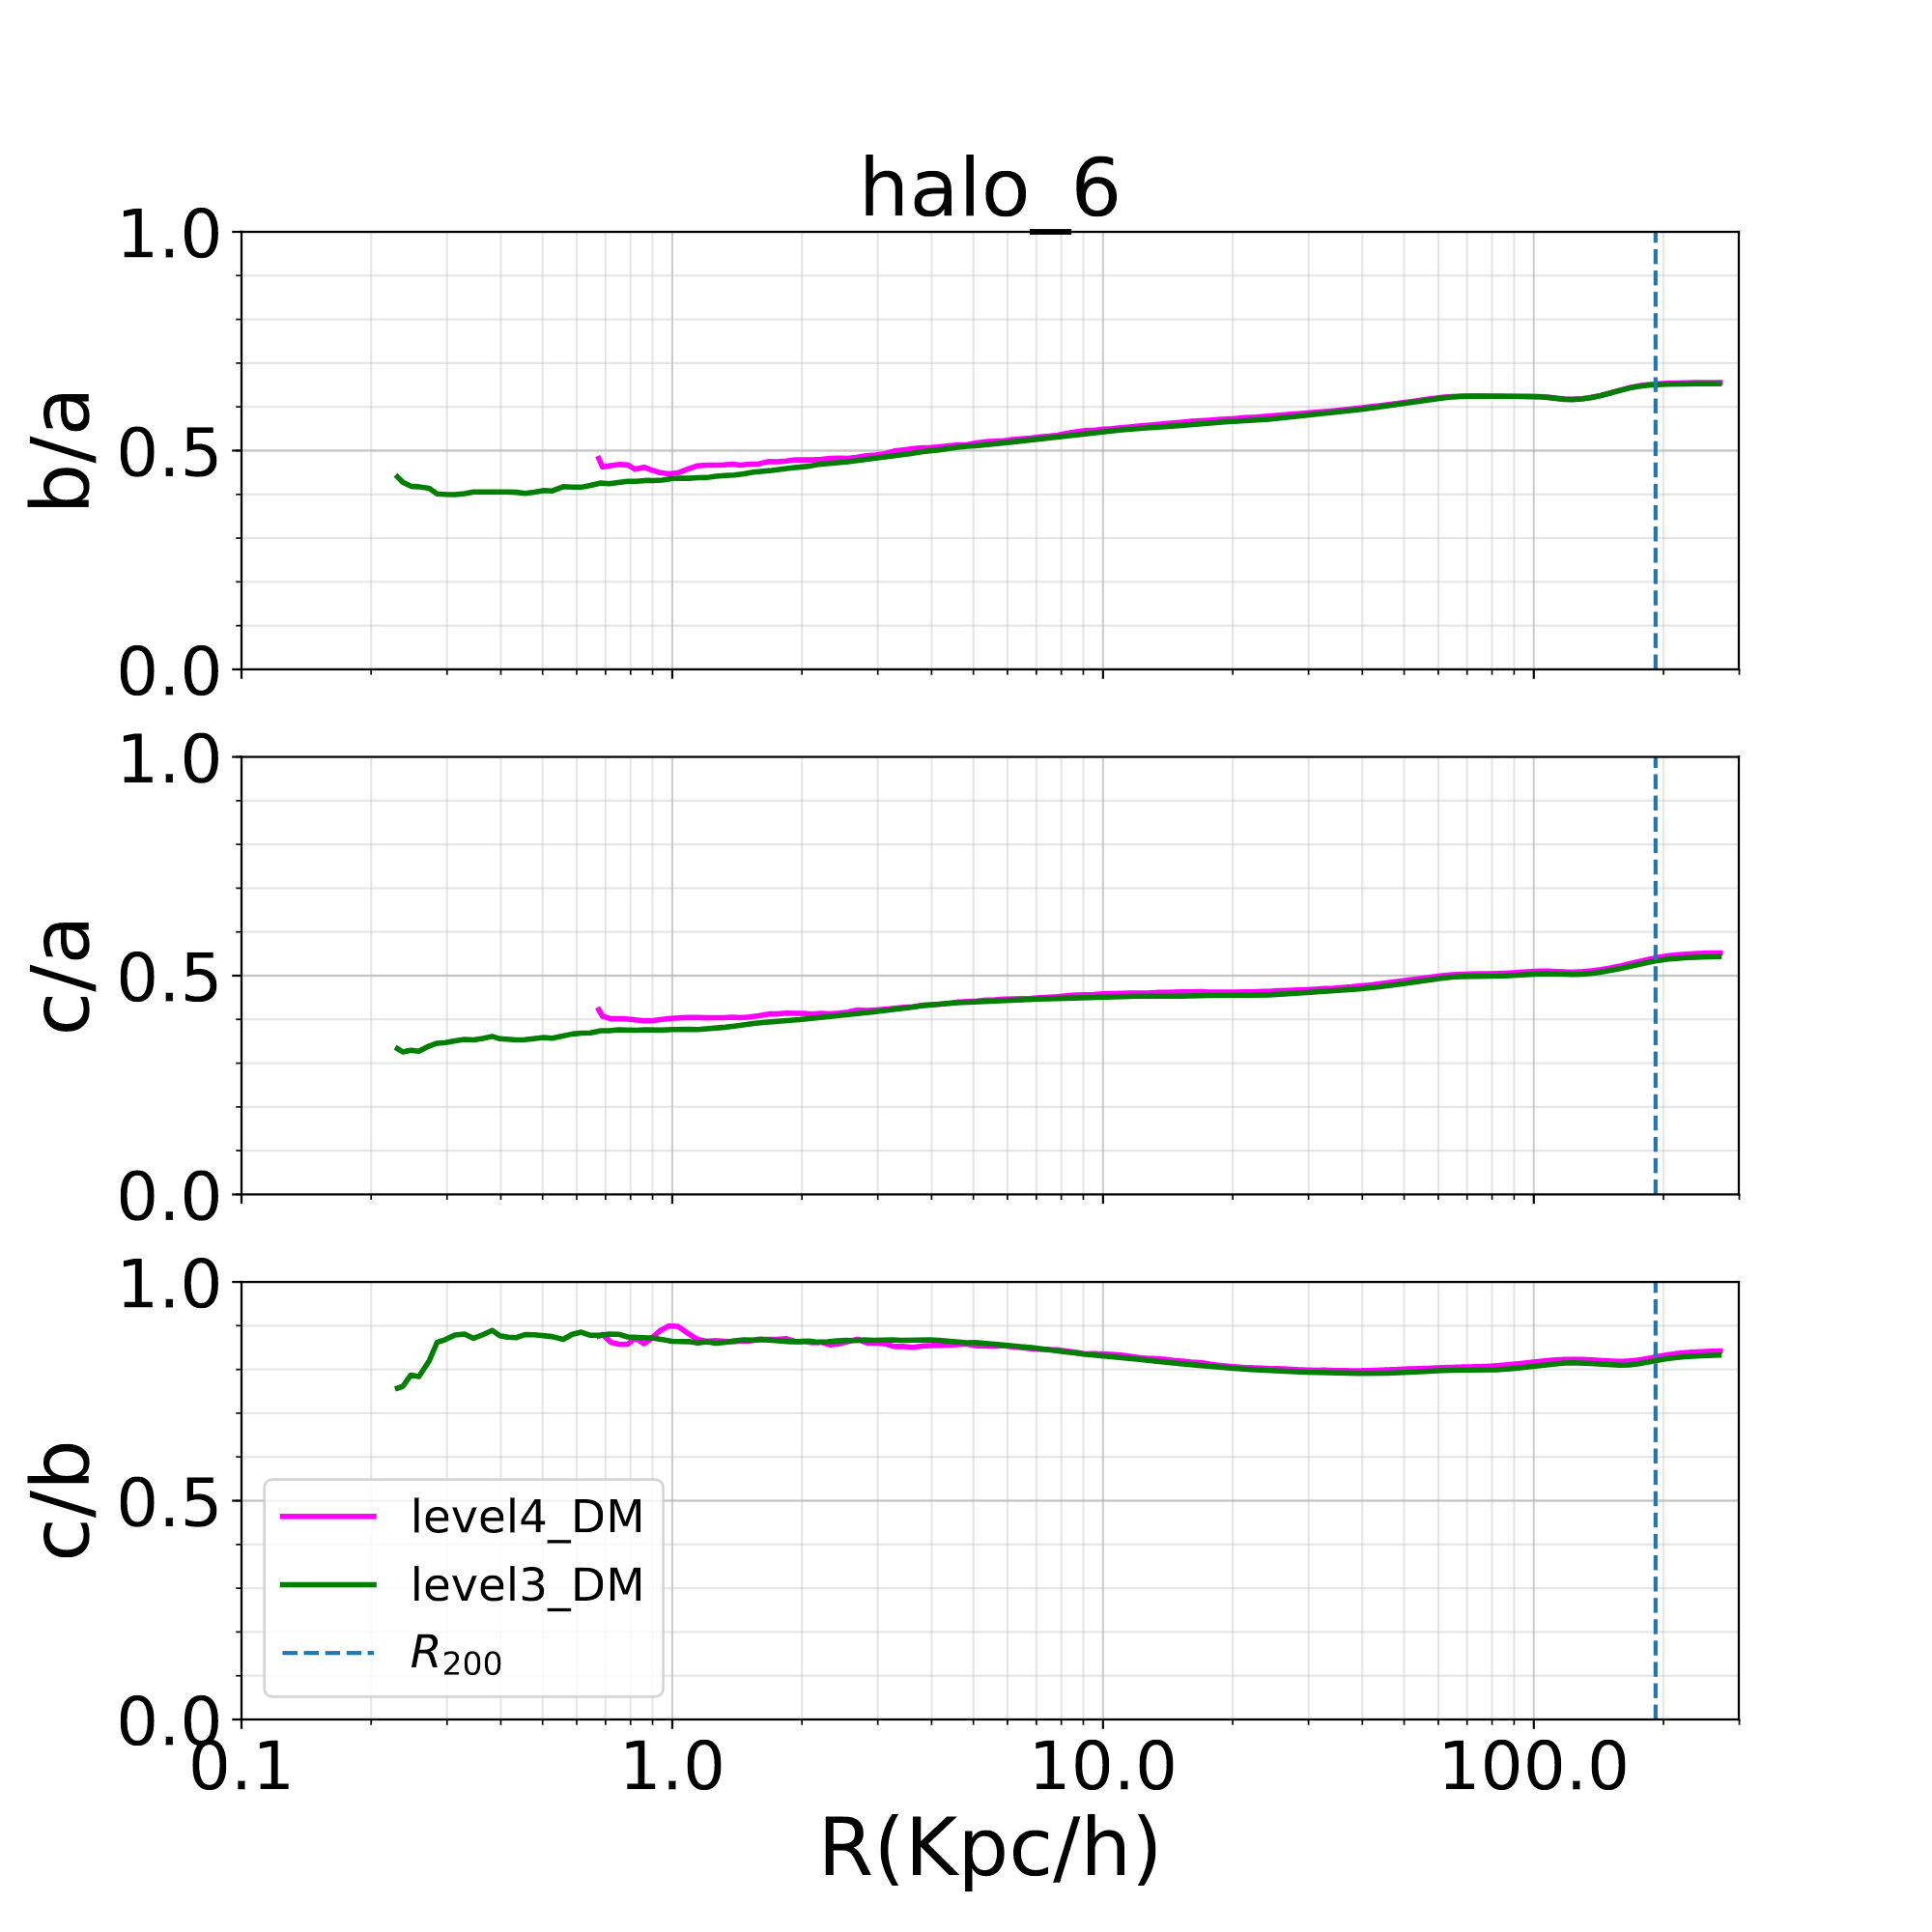
\includegraphics[width=0.5\columnwidth]{./pics/Convergence/halo6_DM_3Vs4_good.png}\label{fig:goodConvergenceDM}}
  \hfill
  \subfloat[halo 27 DM]{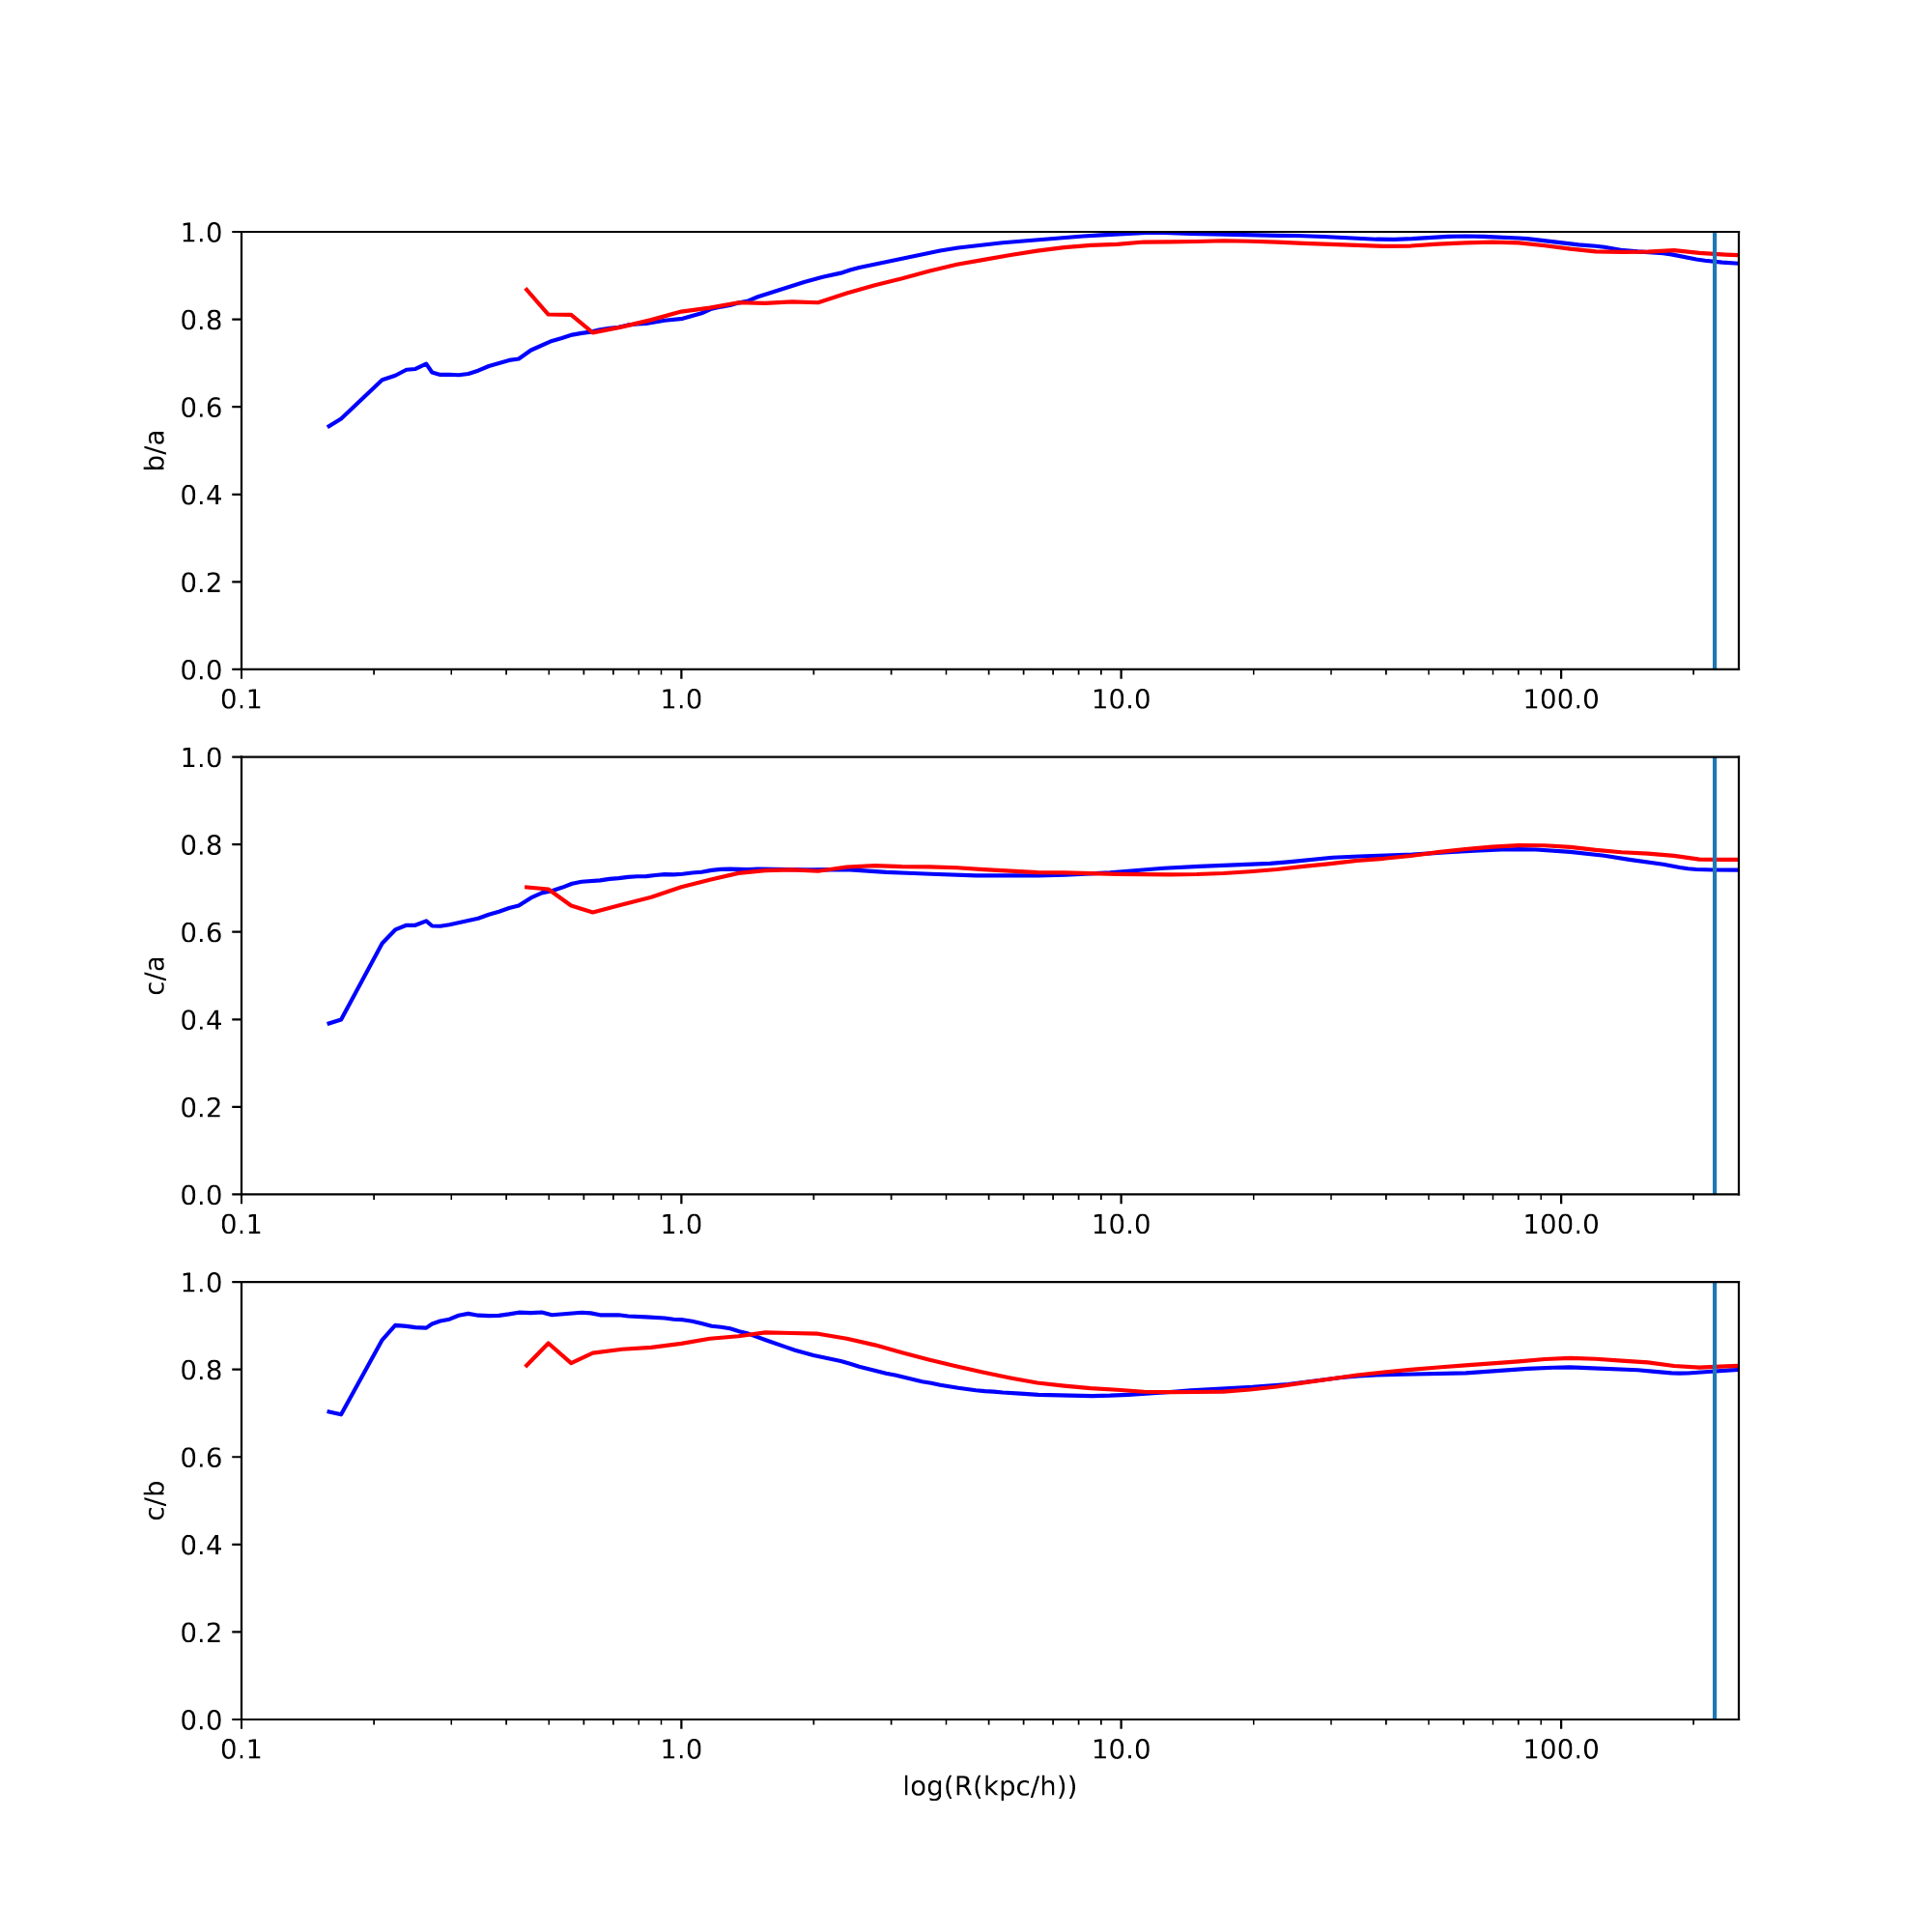
\includegraphics[width=0.5\columnwidth]{./pics/Convergence/halo27_MHD_3Vs4_good.png}\label{fig:goodConvergenceMHD}}
  \caption{Examples of halos where resolution did not have an appreciable effect on the halo shape. Level 3 (blue) and level 4 (red) calculations are in good agreement. \textbf{put labels, bigger axes font, add title} }
\end{figure}



\begin{figure}[!ht]
  \centering
  \subfloat[halo_21 MHD]{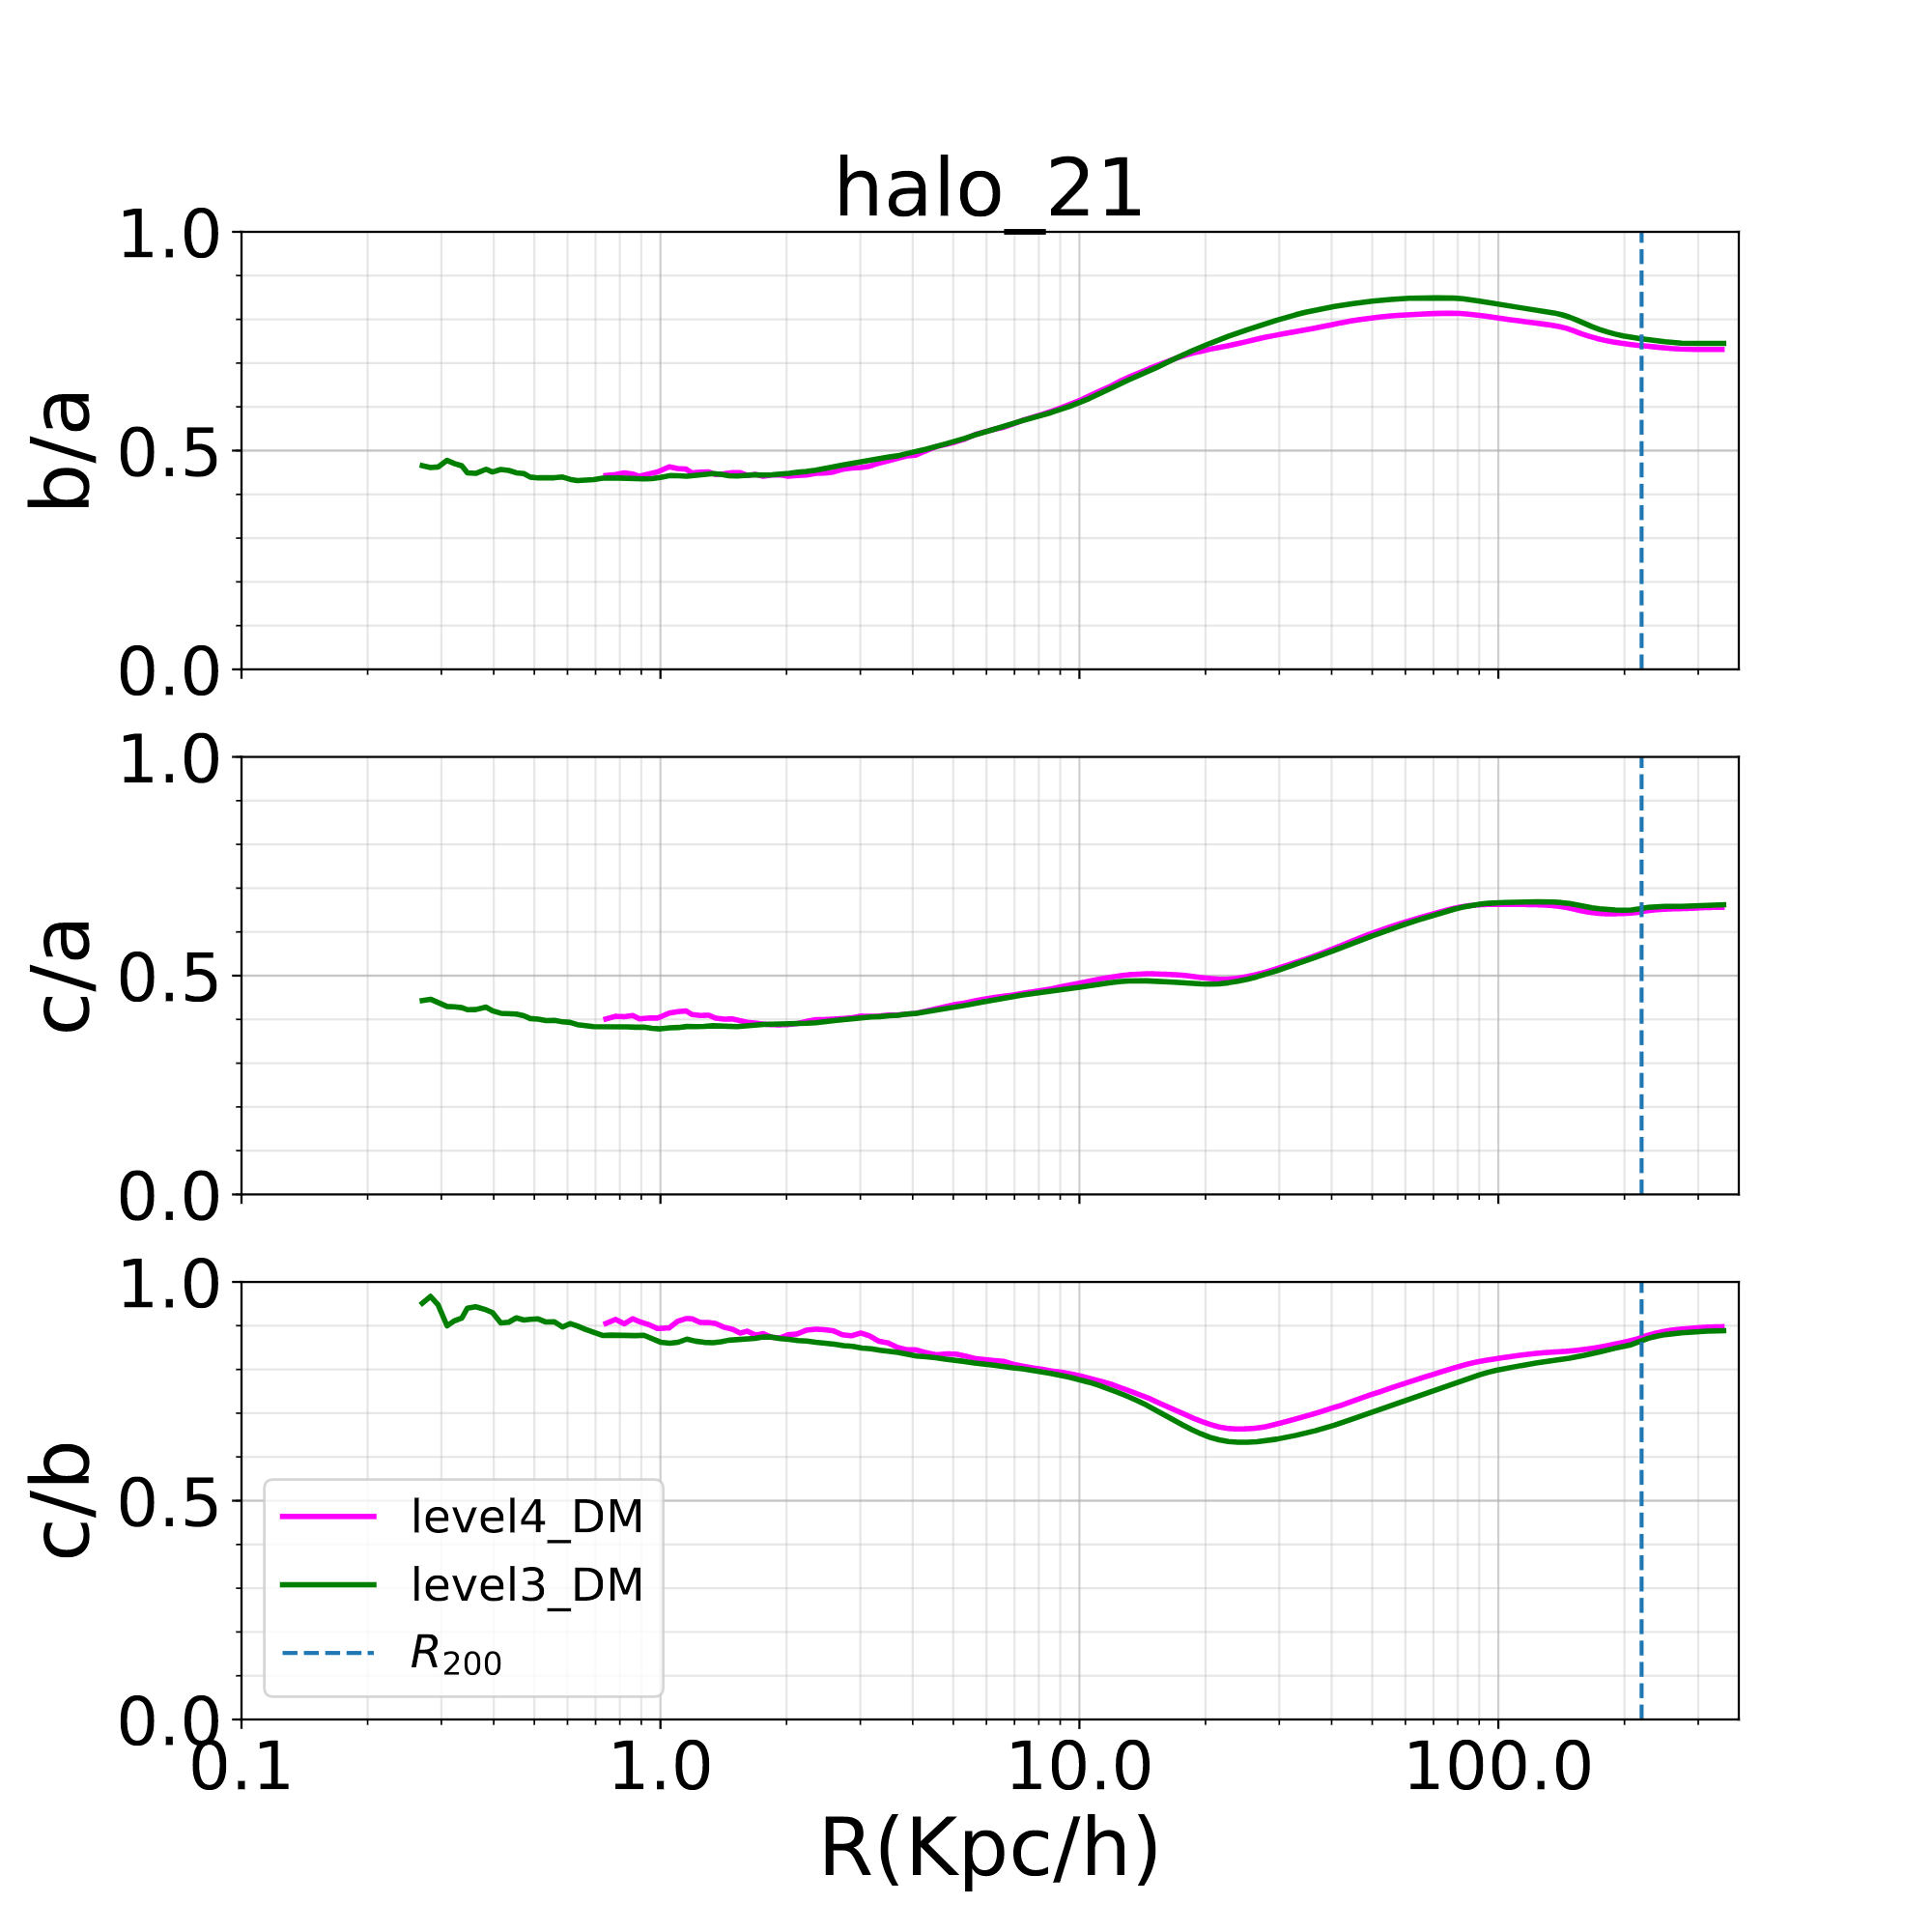
\includegraphics[width=0.5\columnwidth]{./pics/Convergence/halo21_DM_3Vs4_bad.png}\label{fig:badConvergenceDM}}
  \hfill
  \subfloat[halo_23 DM]{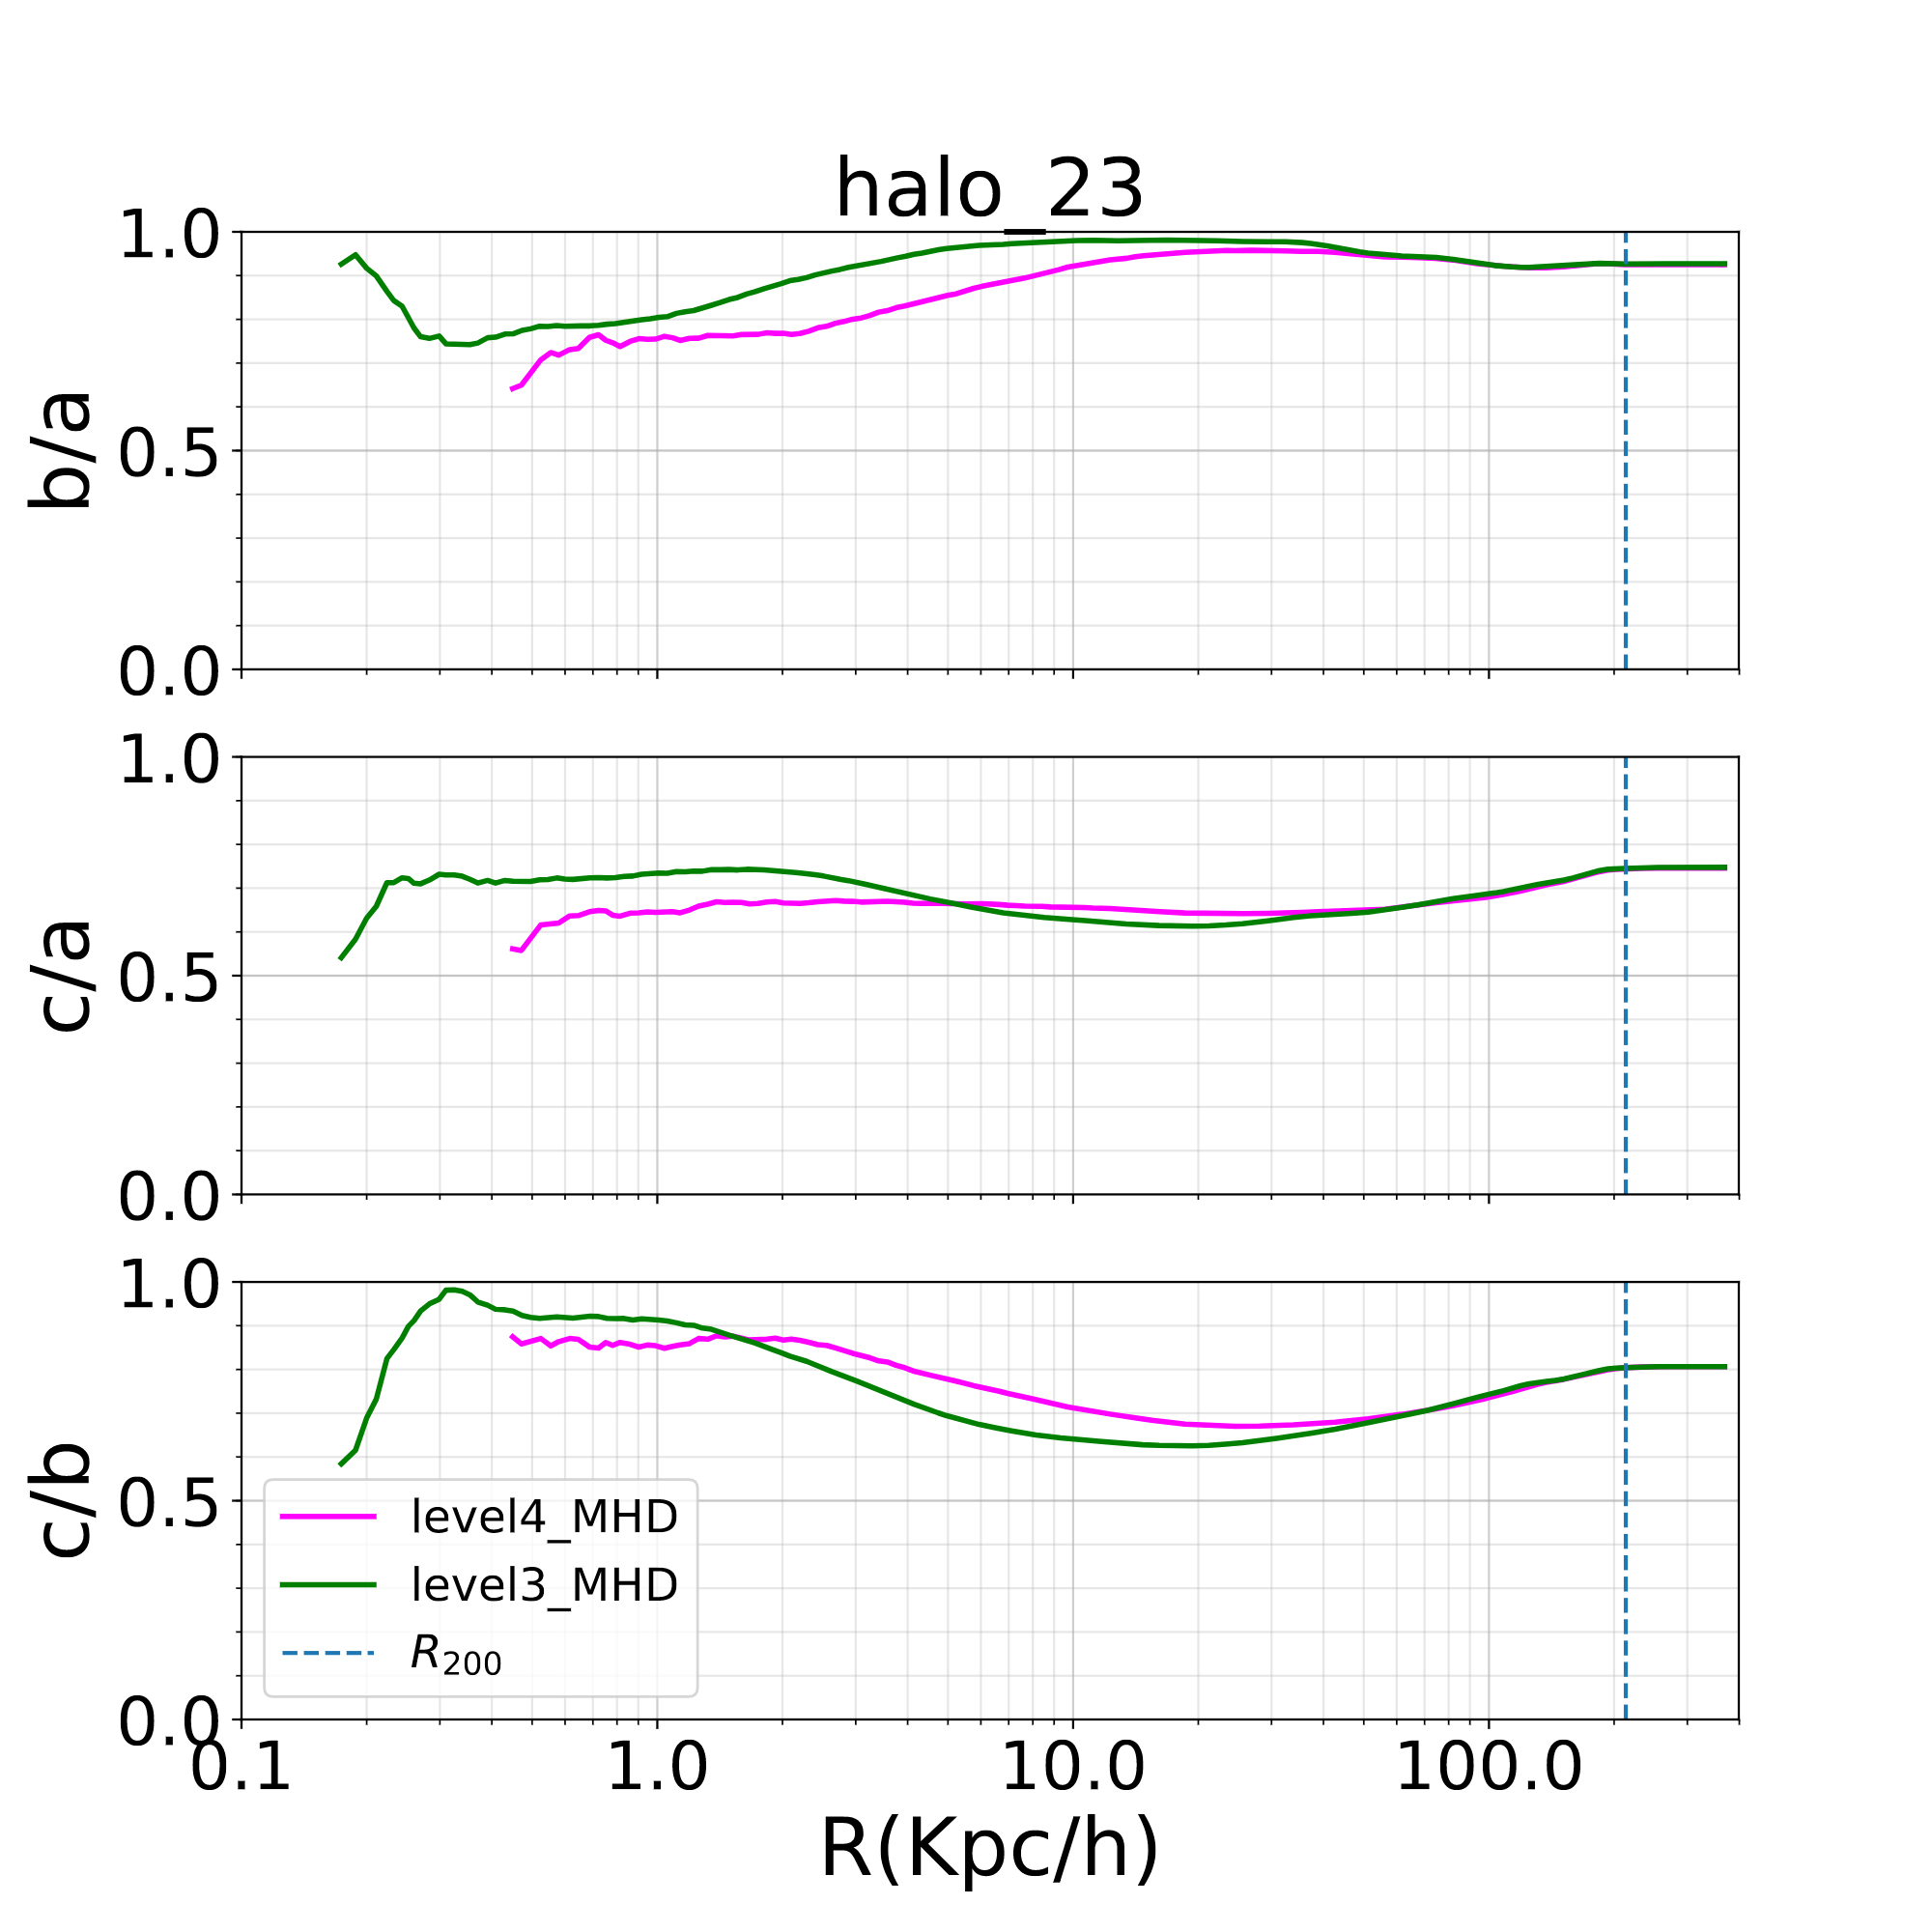
\includegraphics[width=0.5\columnwidth]{./pics/Convergence/halo23_MHD_3Vs4_bad.png}\label{fig:badConvergenceMHD}}
  \caption{Examples of halos where resolution had an appreciable effect on the halo shape. There is an appreciable difference between level 3 (blue) and level 4 (red) calculations. However it does not modify the halo's shape in any specific way. \textbf{put labels, bigger axes font, add title} }
\end{figure}


We decided to analyze de radial profiles at redshift 0 and compare level5 to level3 simulations. In general, the DM halo shapes remain unchanged with the exeption of the radial regimes where resolution becomes important. However, for MHD simulations, the resolution of gas affects the measurement not only in the inner parts, where resolution issues are evident, but it has a more global effect, presumably because of the scattering of particles which is also supporting the claim that matter affects the halo shape through scattering.\\

We address this problem by performing random sampling of the level3 simulations to reproduce level4 measurements and estimate the associated error.\\

\begin{figure}[!ht]
  \centering
  \subfloat[halo 24 MHD]{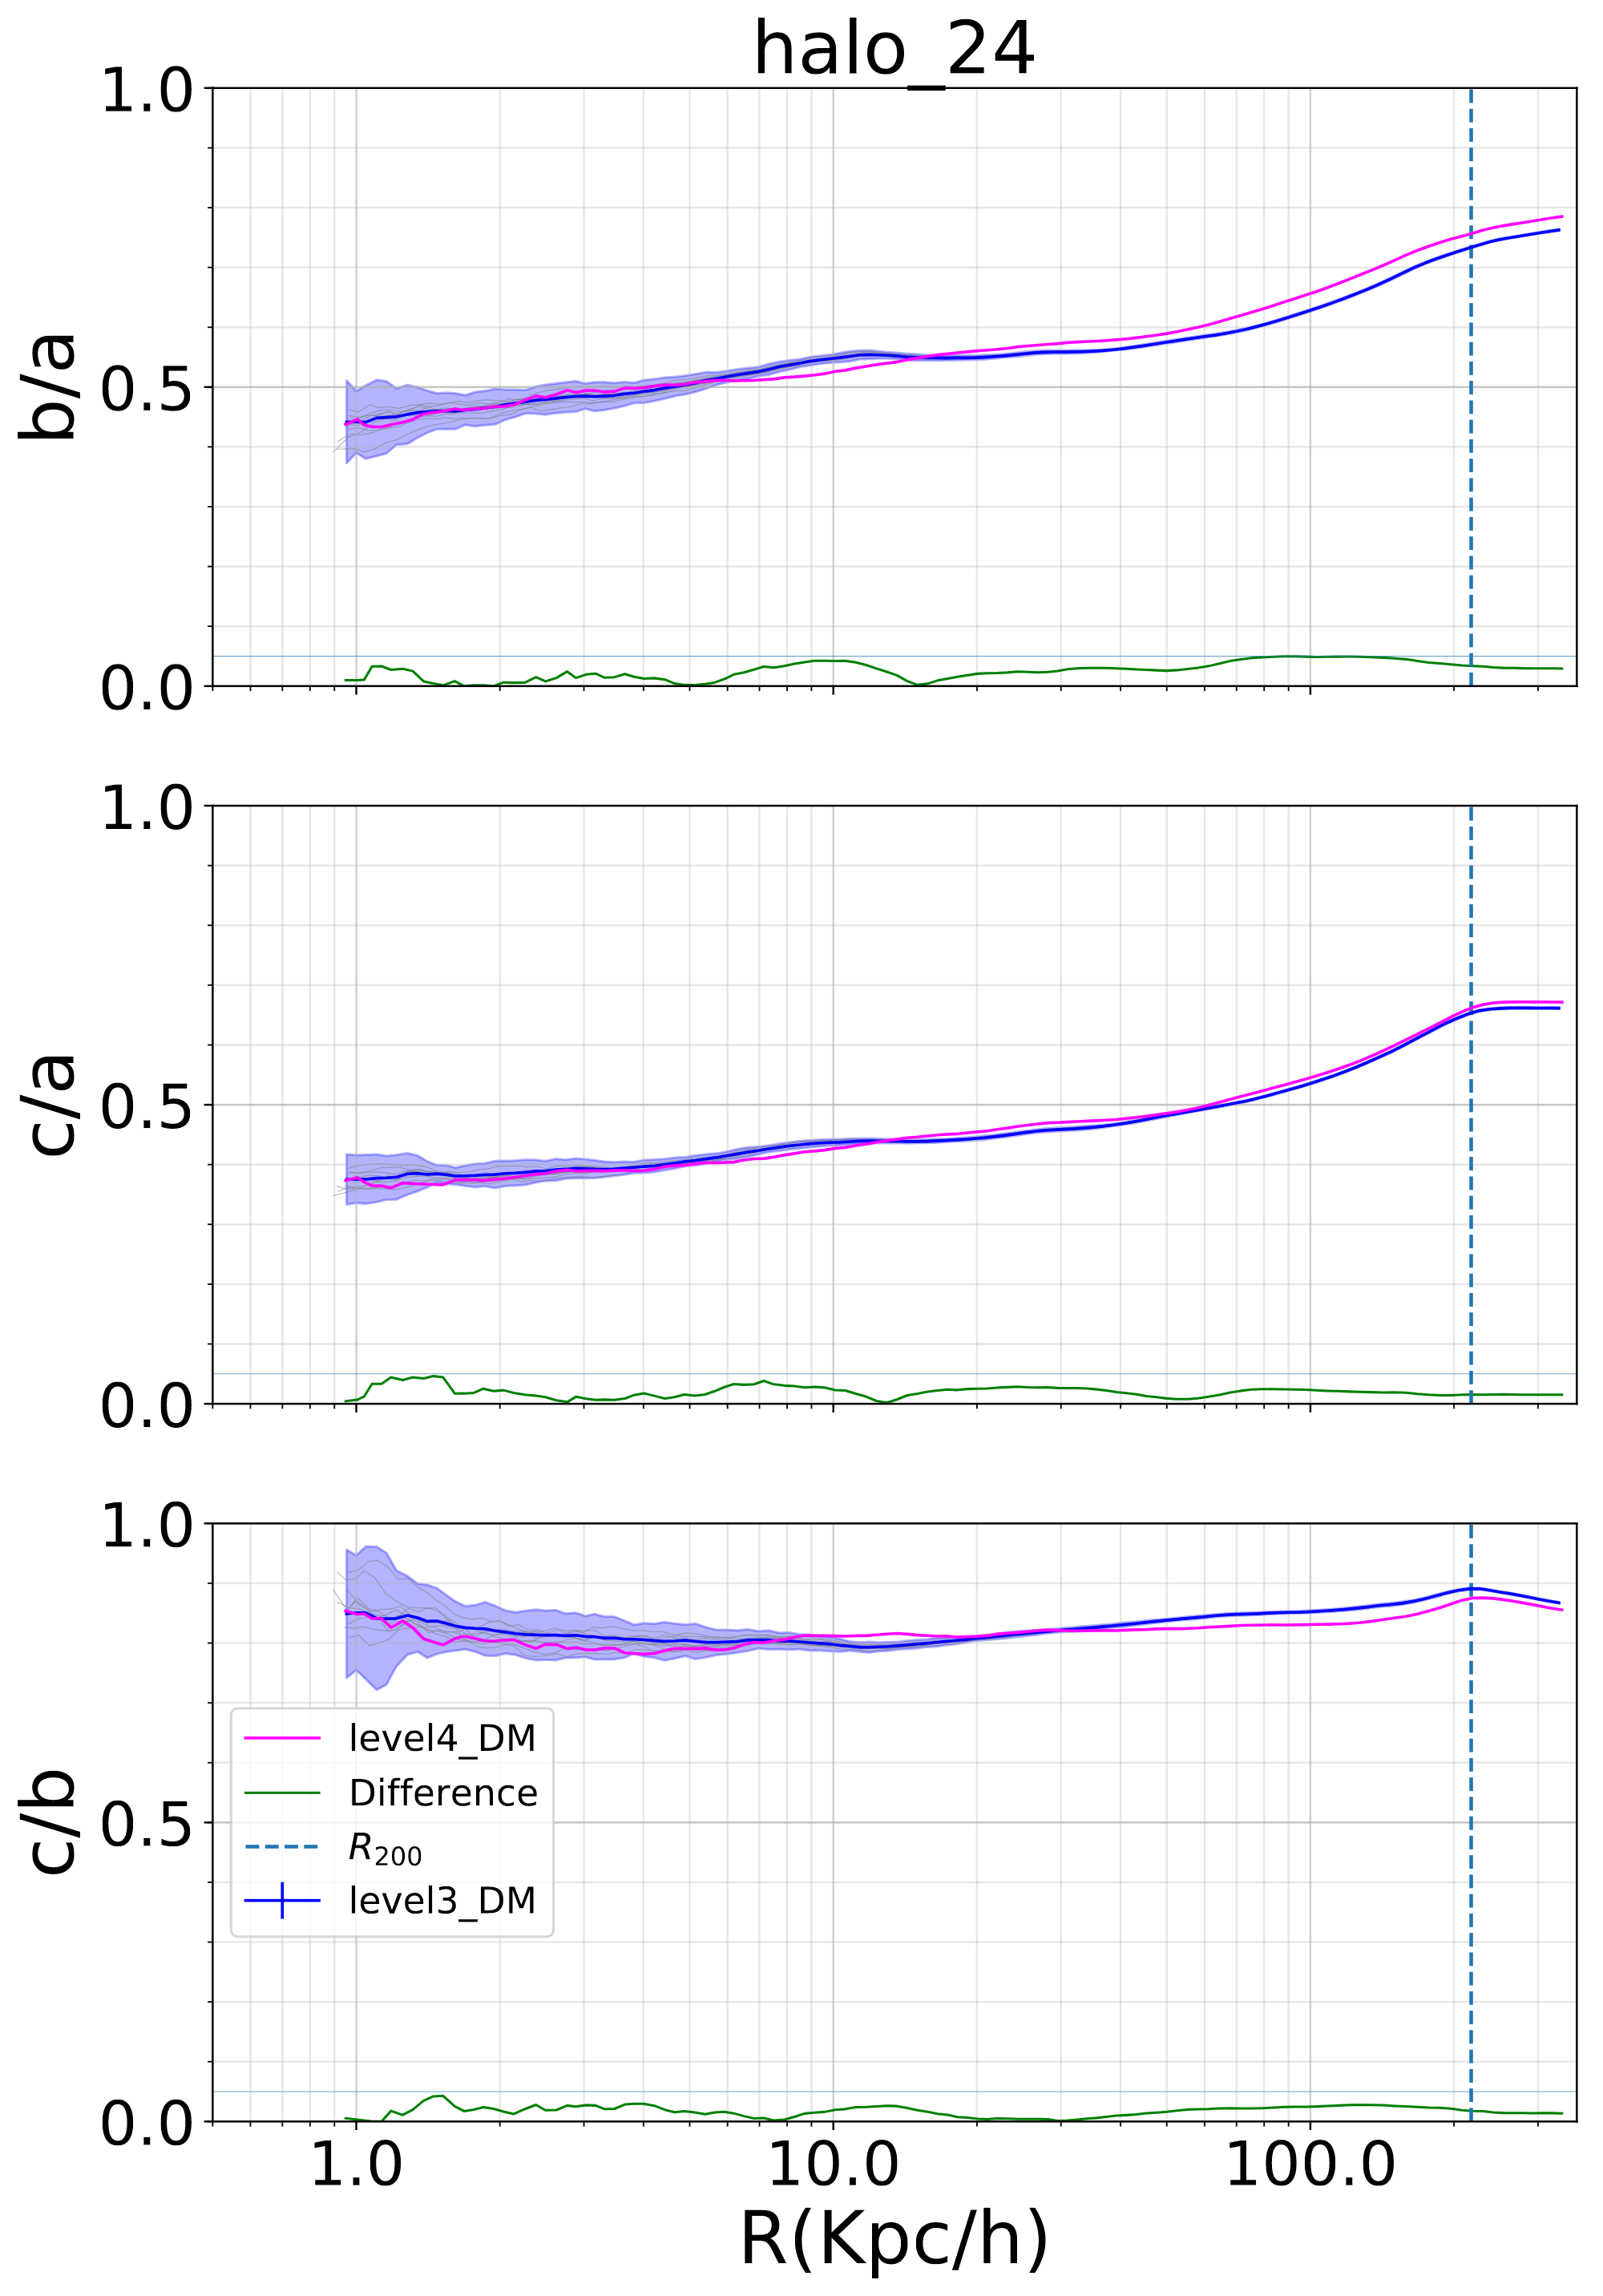
\includegraphics[width=0.5\columnwidth]{./pics/Convergence/rand_conv_halo24_DM.png}\label{fig:convergenceMHD}}
  \hfill
  \subfloat[halo 24 DM]{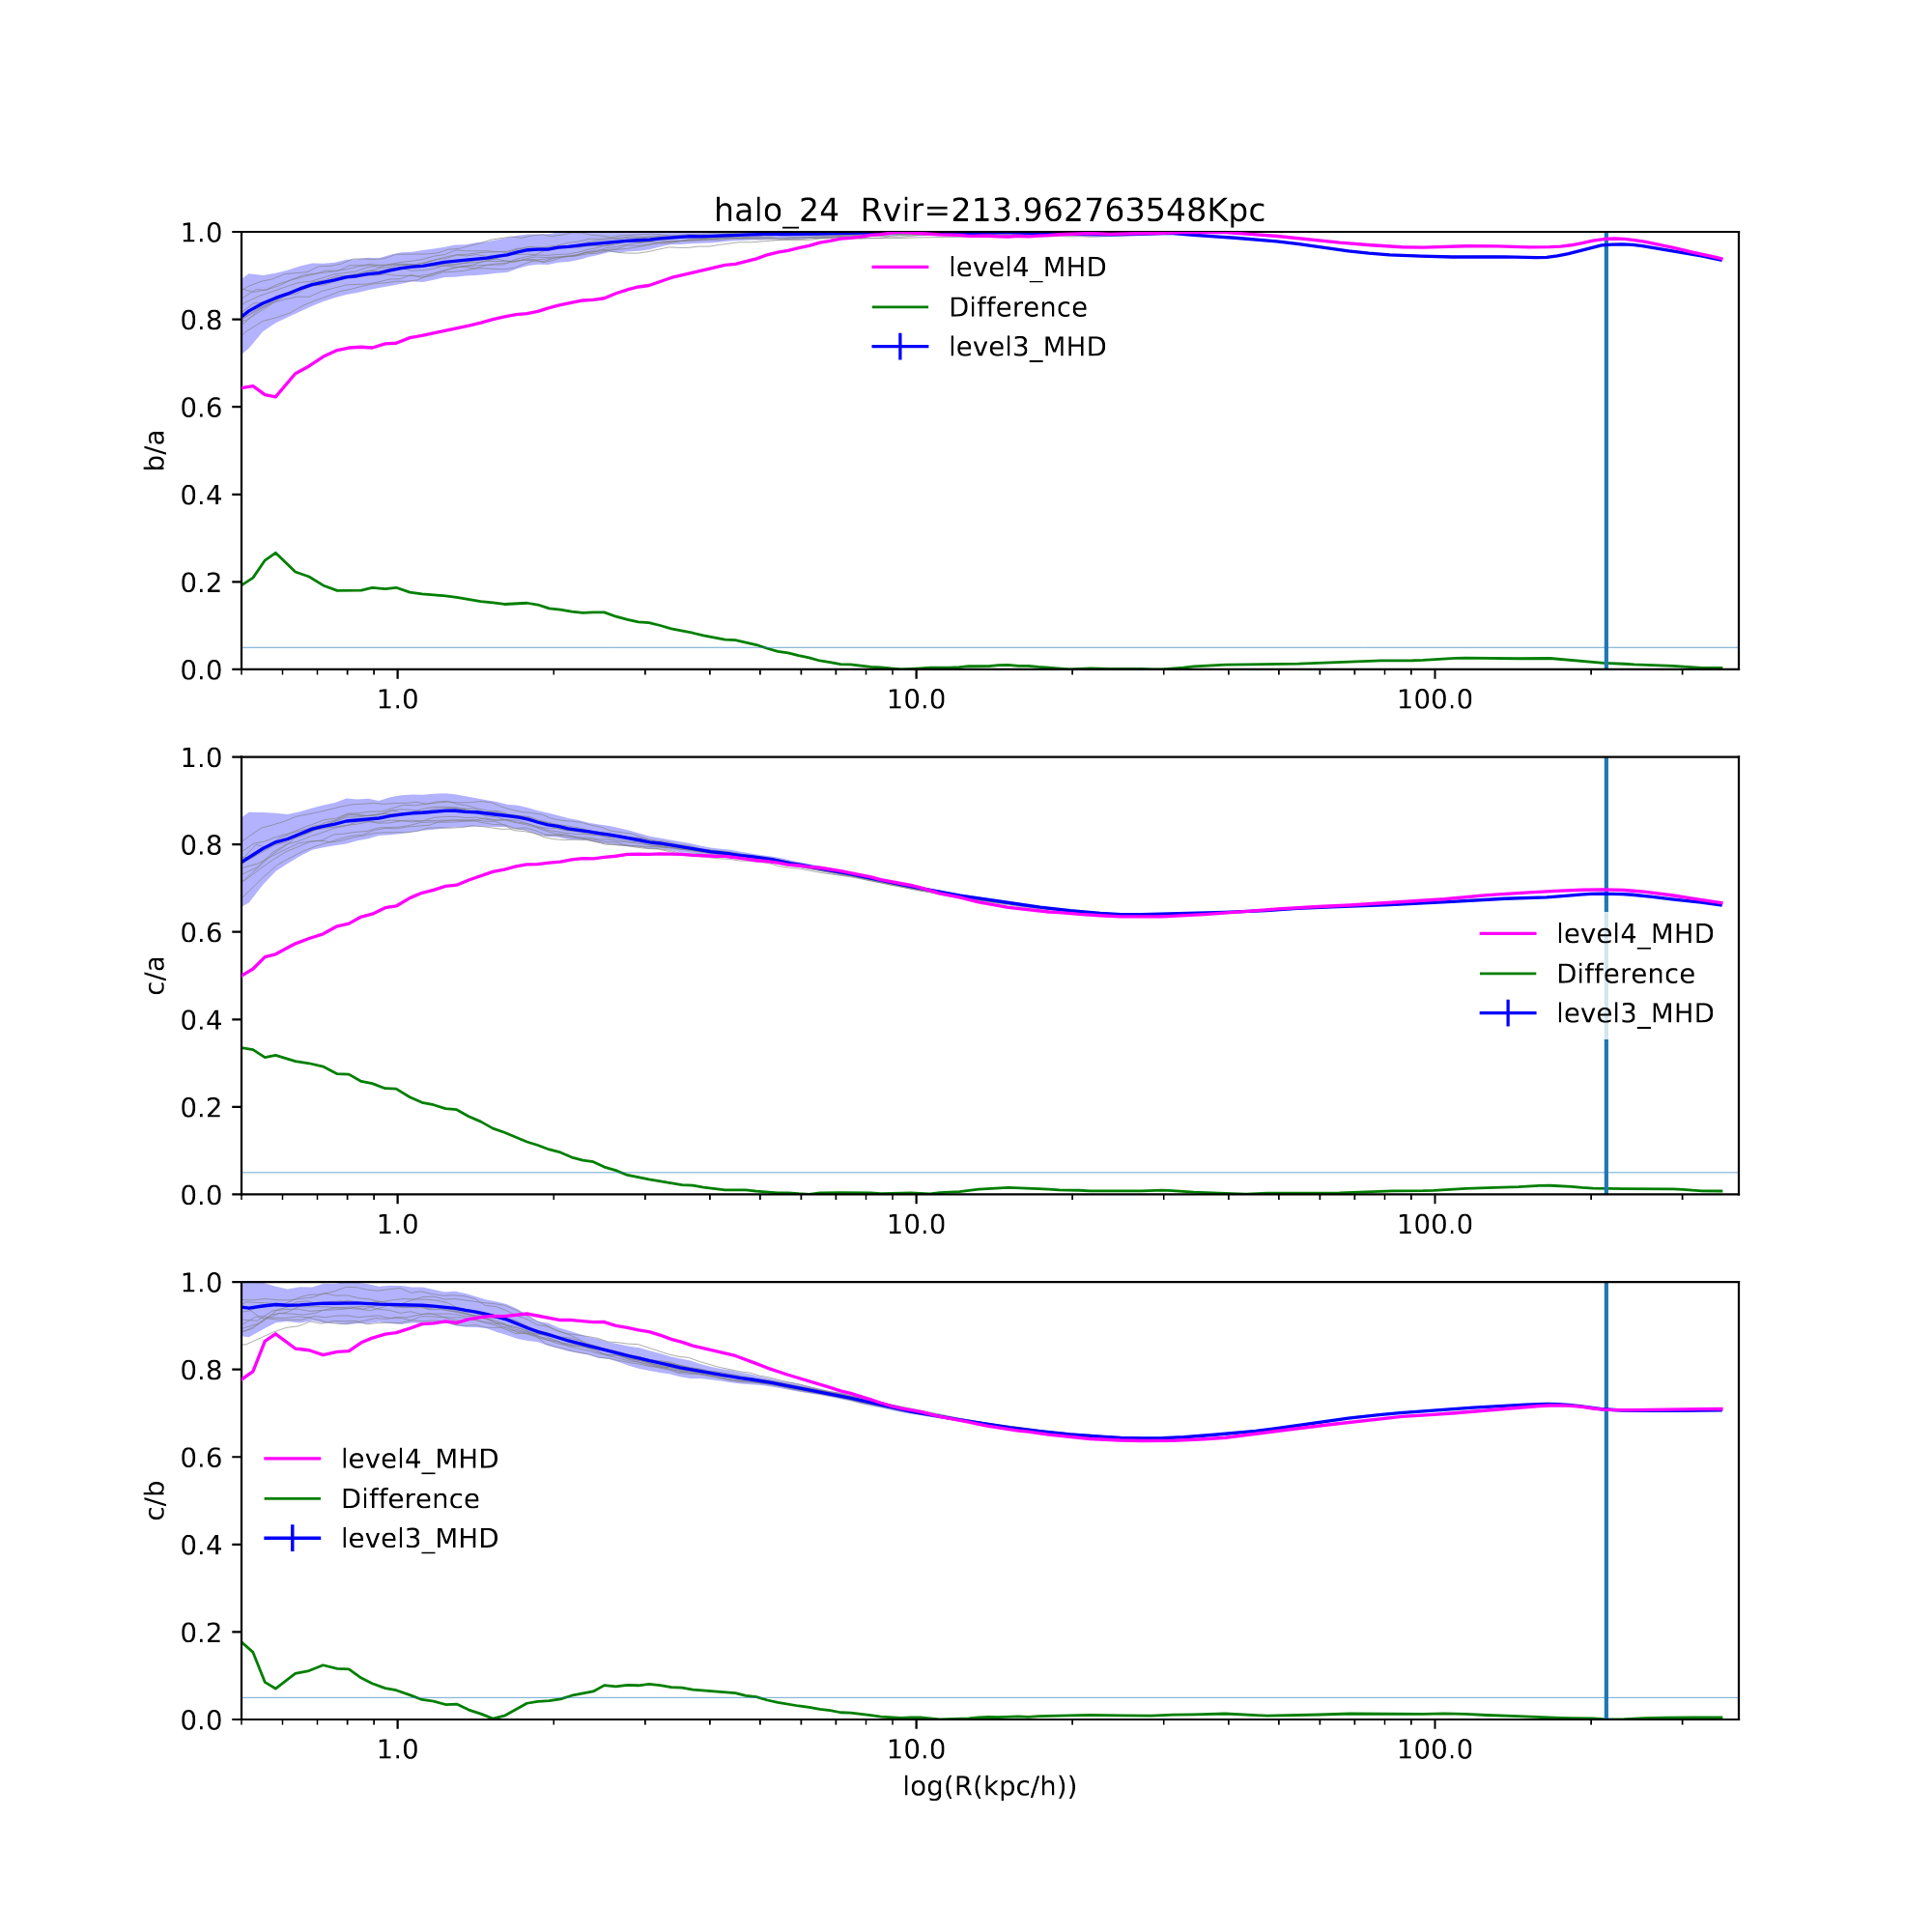
\includegraphics[width=0.5\columnwidth]{./pics/Convergence/rand_conv_halo24_MHD.png}\label{fig:convergenceDM}}
  \caption{Comparison of the effect of resolution on DM and MHD simualations. Here level4 curves (magenta) are compared to the mean and 2std (confirm) of the random-sampled curves from level3. For better comparison of the effect of resolution, the difference percent is plotted in green.  \textbf{bigger axes font}}
\end{figure}



State the main conclusions about this analysis of convergence. The effect of particle resolution does not sistematically affect the measurements. However, the error produced is specially apreciable at inner parts where for MHD it has a more global effect through scattering.\\

Halo shape is heavily determined by accretion with environment \cite{shape relation with environment}. As environment may also be affected by resolution, this may have an effect on the halo shape. Also, resolution discrepancies may snowball through history.

\section{The shape's radial dependence}
One of the first results we obtained in this work is related to the impact of the radius on the shape. Halos accrete mass from inner shells to outter shells. Inner shells are isolated from outter regions (gauss law effect?) and tend to conserve their shape (angular momentum?). Outter shells, on the other side are affected by the inner gravitational potential and is prone to scattering effects. This has a "rounding" effect on the halo shape. For this reason, we expect on both simulations (lvl3MHD,lvl3DM) that halos are more triaxial on inner regions and more spherical at bigger radii.\\


\begin{figure}[!ht]
  \centering
  \subfloat[halo 27 DM shape at small radius]{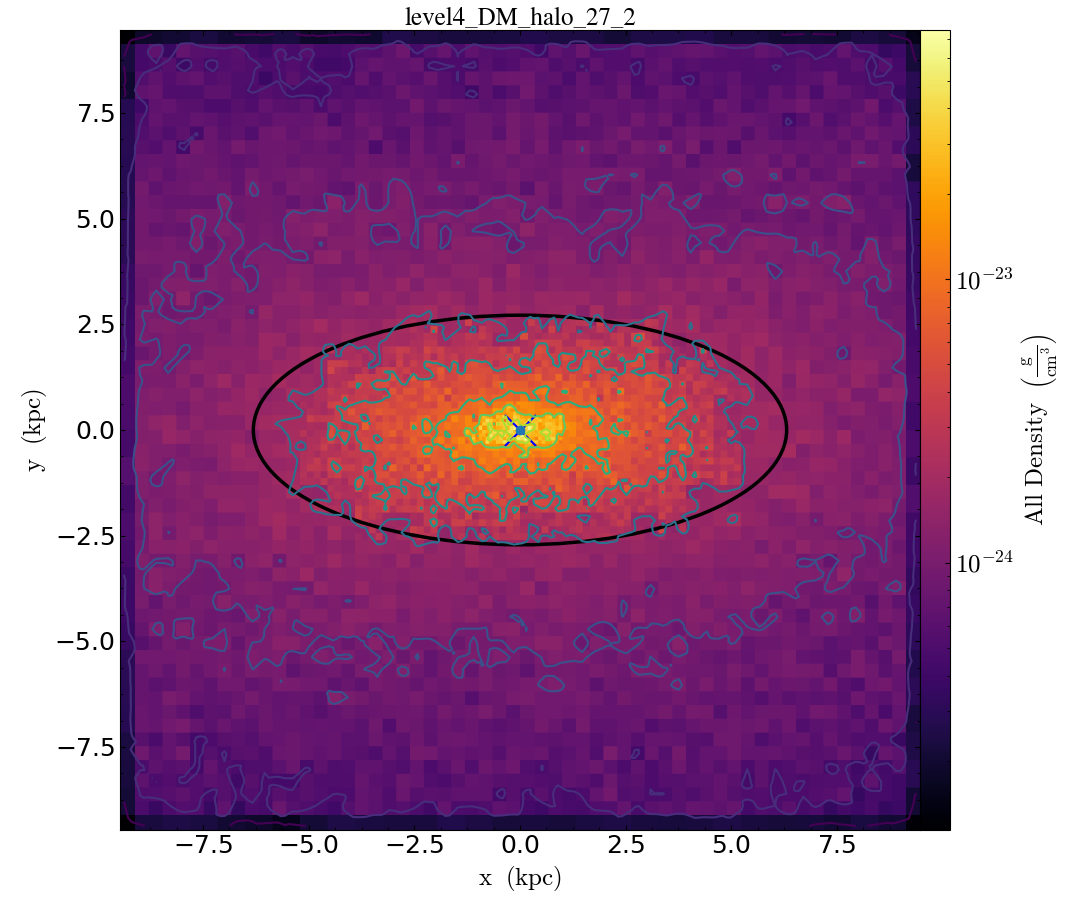
\includegraphics[width=0.5\columnwidth]{./pics/MHD_Vs_DM/level4_DM_halo_27_inner.png}\label{fig:innerDM}}
  \hfill
  \subfloat[halo 27 DM shape at big radius]{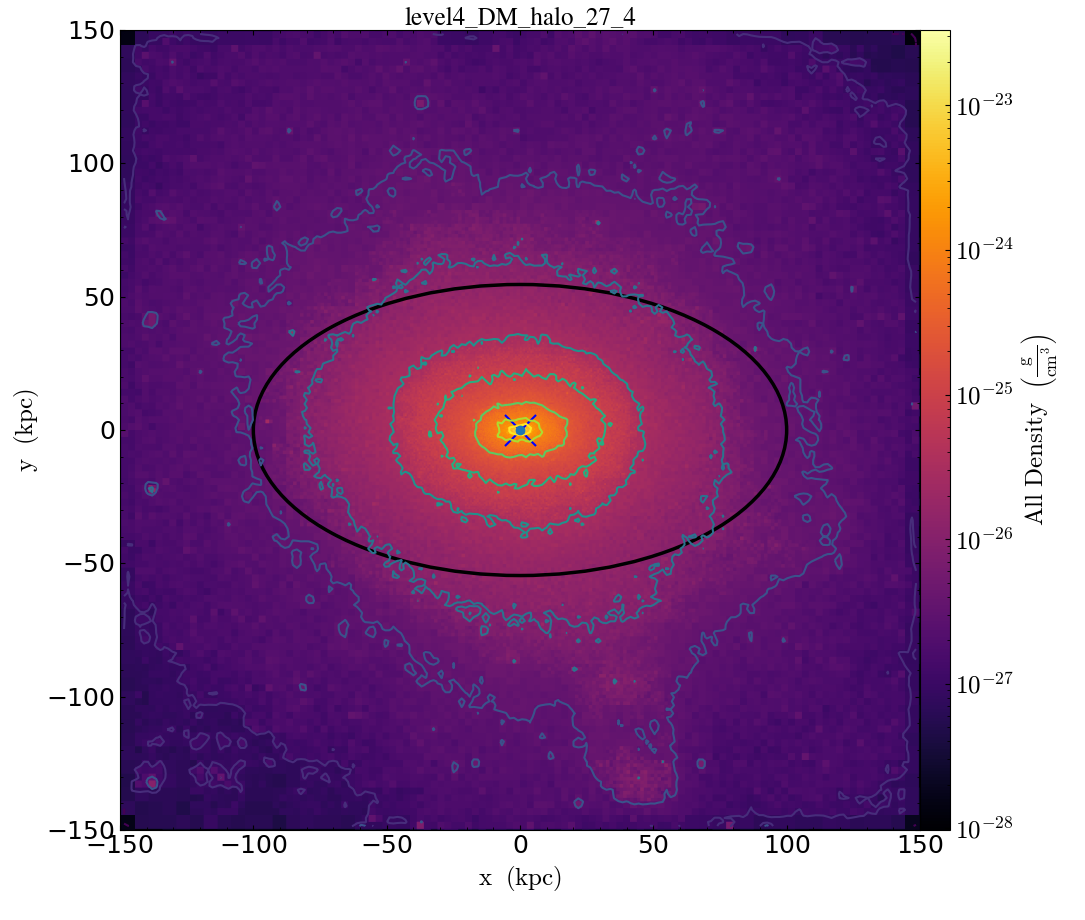
\includegraphics[width=0.5\columnwidth]{./pics/MHD_Vs_DM/level4_DM_halo_27_outter.png}\label{fig:outterDM}}
  \hfill
  \subfloat[halo 27 MHD shape at small radius]{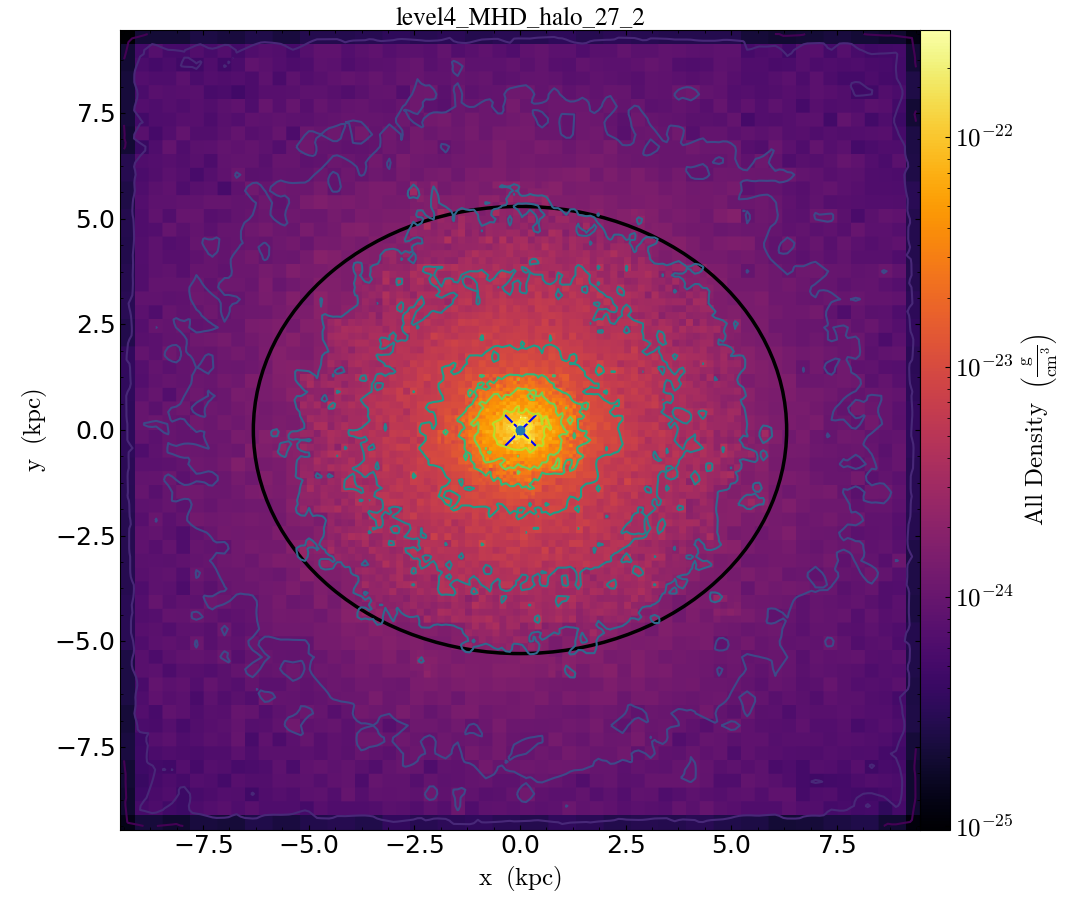
\includegraphics[width=0.5\columnwidth]{./pics/MHD_Vs_DM/level4_MHD_halo_27_inner.png}\label{fig:innerMHD}}
  \hfill
  \subfloat[halo 27 MHD shape at big radius]{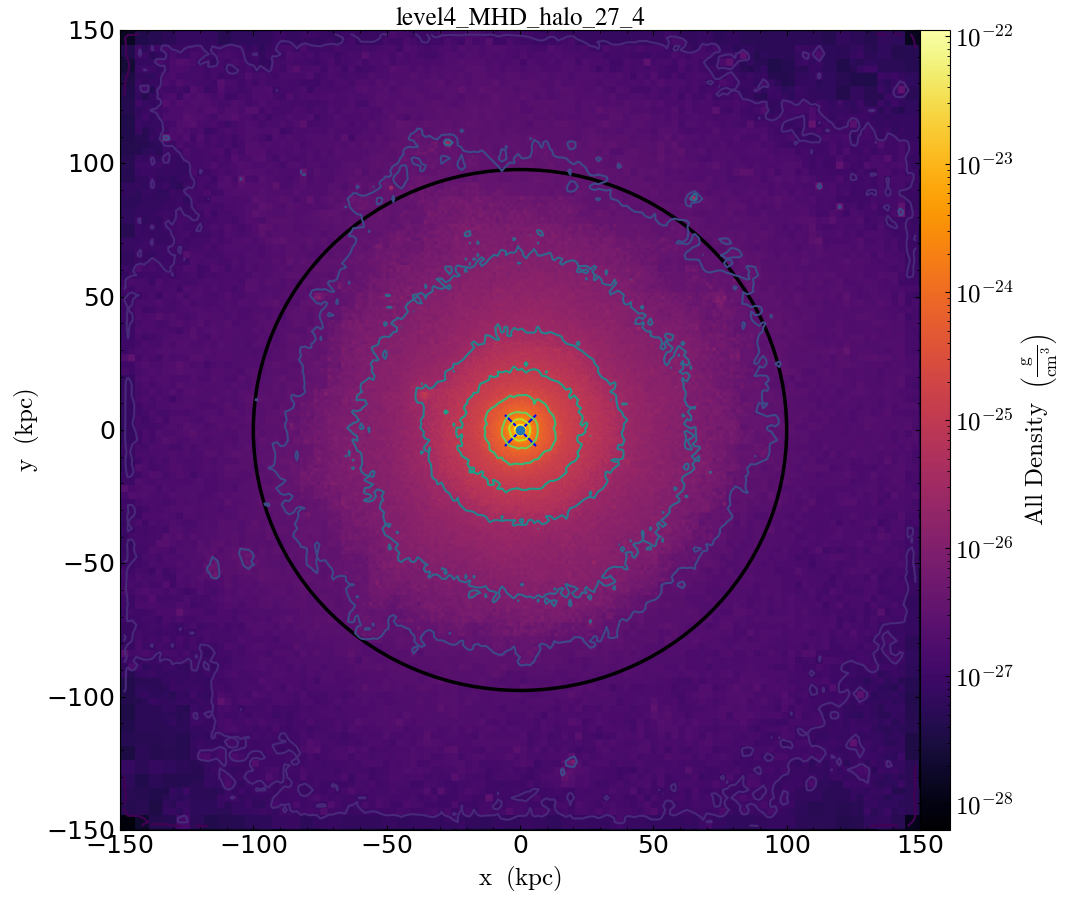
\includegraphics[width=0.5\columnwidth]{./pics/MHD_Vs_DM/level4_MHD_halo_27_outter.png}\label{fig:outterMHD}}
  \caption{Example of the dependence of shape in terms of the radius. All graphics have matching orientation (which may not be the same) with their respective principal axes at the shown radii. The horizontal and vertical axes correspond to the major and medium semi-axes respectively. }
\end{figure}

\subsection{The effect of gas on the halo shape}
The rounding effect with radius is specially evident in this example, but it is a general tendency over all. From this comparison we can notice that there is also a relation of this roundong effect with the presence of matter, which is to be expected. Unlike DM, gas collapses and generate disks which are much denser than DM at the scales where it forms. This amplifies scattering events and if we apply the same logic, we would expect that the inner regions of the halo are more spherical when there is presence of DM. We expect the same for outter regions but this effect is expected to be more significant due to the stronger effect of the gravitational potential on the outter shells.\\

\begin{figure}
\centering
{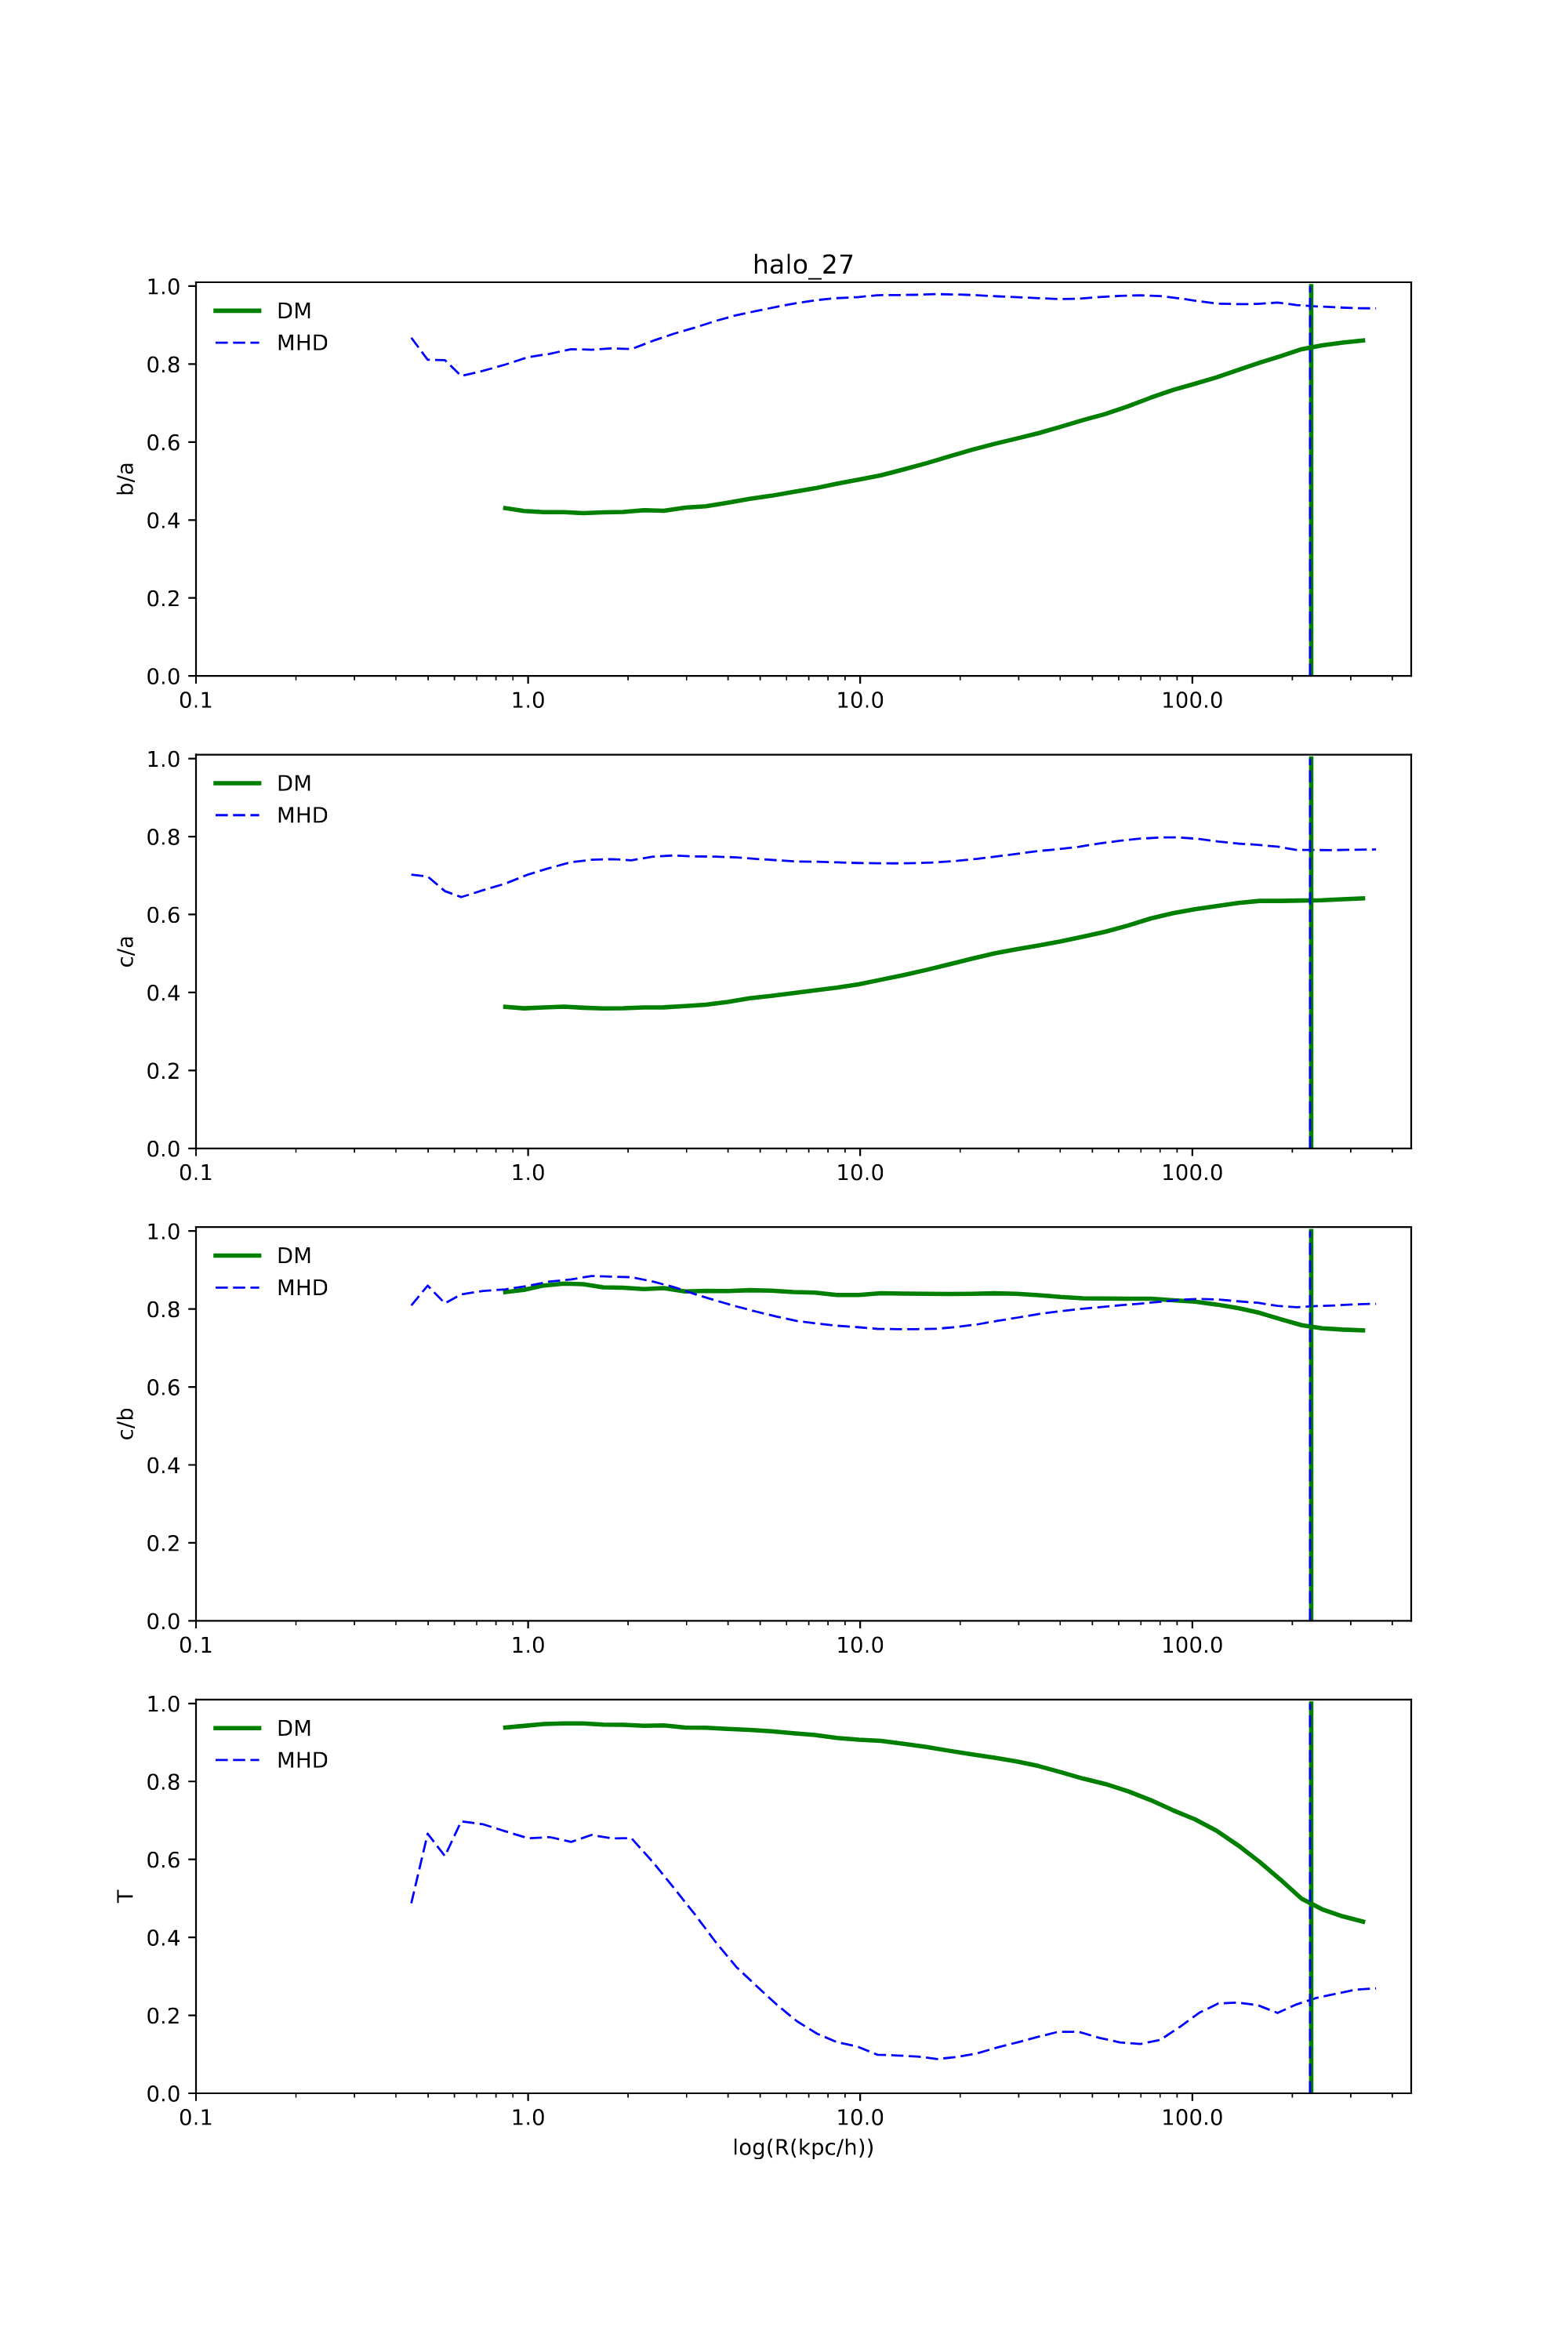
\includegraphics[width=1\columnwidth]{./pics/MHD_Vs_DM/level4_halo_27_DM_Vs_MHD.png}\label{fig:outterMHD}}
\caption{Semi-axial ratios and triaxiality $\frac{1-b/a}{1-c/a}$ as function of radius for semi-axes $a\geq b\geq c$. The MHD simulation (blue dotted line) shows ratios closer to $1$ than those from the DM-only (green solid line) simulation. The rounding effect with radius for each simulation separatedly is also well-appreciable in this graphic. The radial-rounding, as well as the gas-presence amplification can be evidenced on the triaxiality function. \textbf{show two examples or reorganize subplots to get a square figure, bigger label and axes font}}
\end{figure} 

The general tendency can be better visualized on the triaxial plane (explain what is that).

\begin{figure}[!ht]
  \centering
  \subfloat[Level3 MHD Vs DM at inner regions]{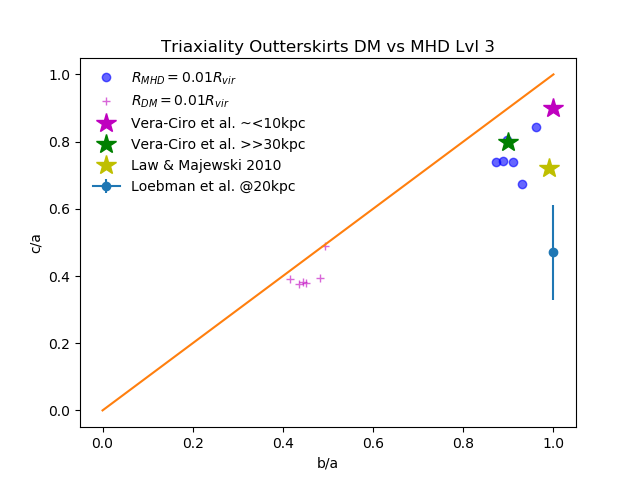
\includegraphics[width=0.5\columnwidth]{./pics/Triaxial_Plane/Triaxiality_Inner_lvl3.png}\label{fig:innerTriaxial3}}
  \hfill
  \subfloat[Level3 MHD Vs DM at outter regions]{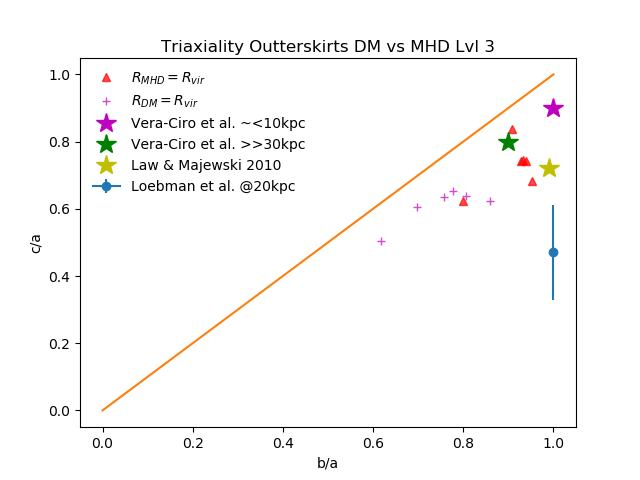
\includegraphics[width=0.5\columnwidth]{./pics/Triaxial_Plane/Triaxiality_Outer_lvl3.png}\label{fig:outterTriaxial3}}
  \hfill
  \centering
  \subfloat[Level4 MHD Vs DM at inner regions]{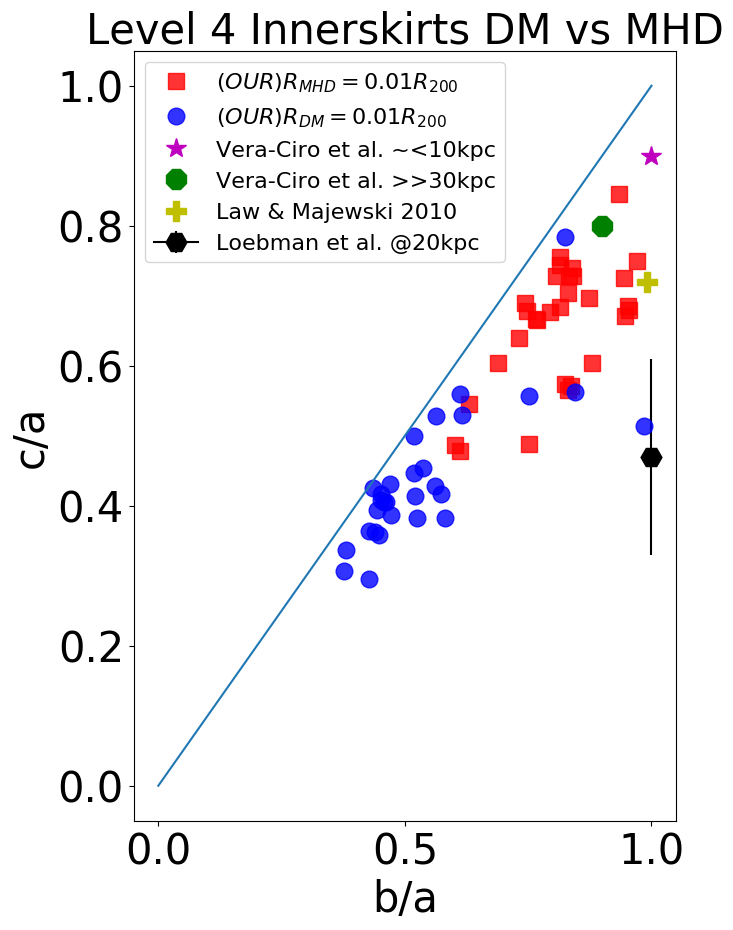
\includegraphics[width=0.5\columnwidth]{./pics/Triaxial_Plane/Triaxiality_Inner_lvl4.png}\label{fig:innerTriaxial4}}
  \hfill
  \subfloat[Level4 MHD Vs DM at outter regions]{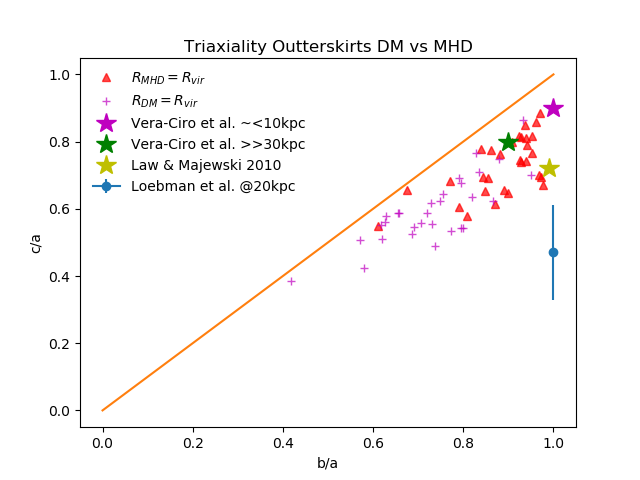
\includegraphics[width=0.5\columnwidth]{./pics/Triaxial_Plane/Triaxiality_Outer_lvl4.png}\label{fig:outterTriaxial4}}
  \hfill
  \caption{General tendence on the triaxial plane $c/a Vs b/a$. Some observational constraints (stars and error-bar point) are plotted alongside our results}
\end{figure}

\section{Historical shape}
Explain why it is expected for the shape to remain more or less constant with time: non-collisional DM, gauss law effect.


\begin{figure}[!ht]
  \centering
  \subfloat[halo 16 DM]{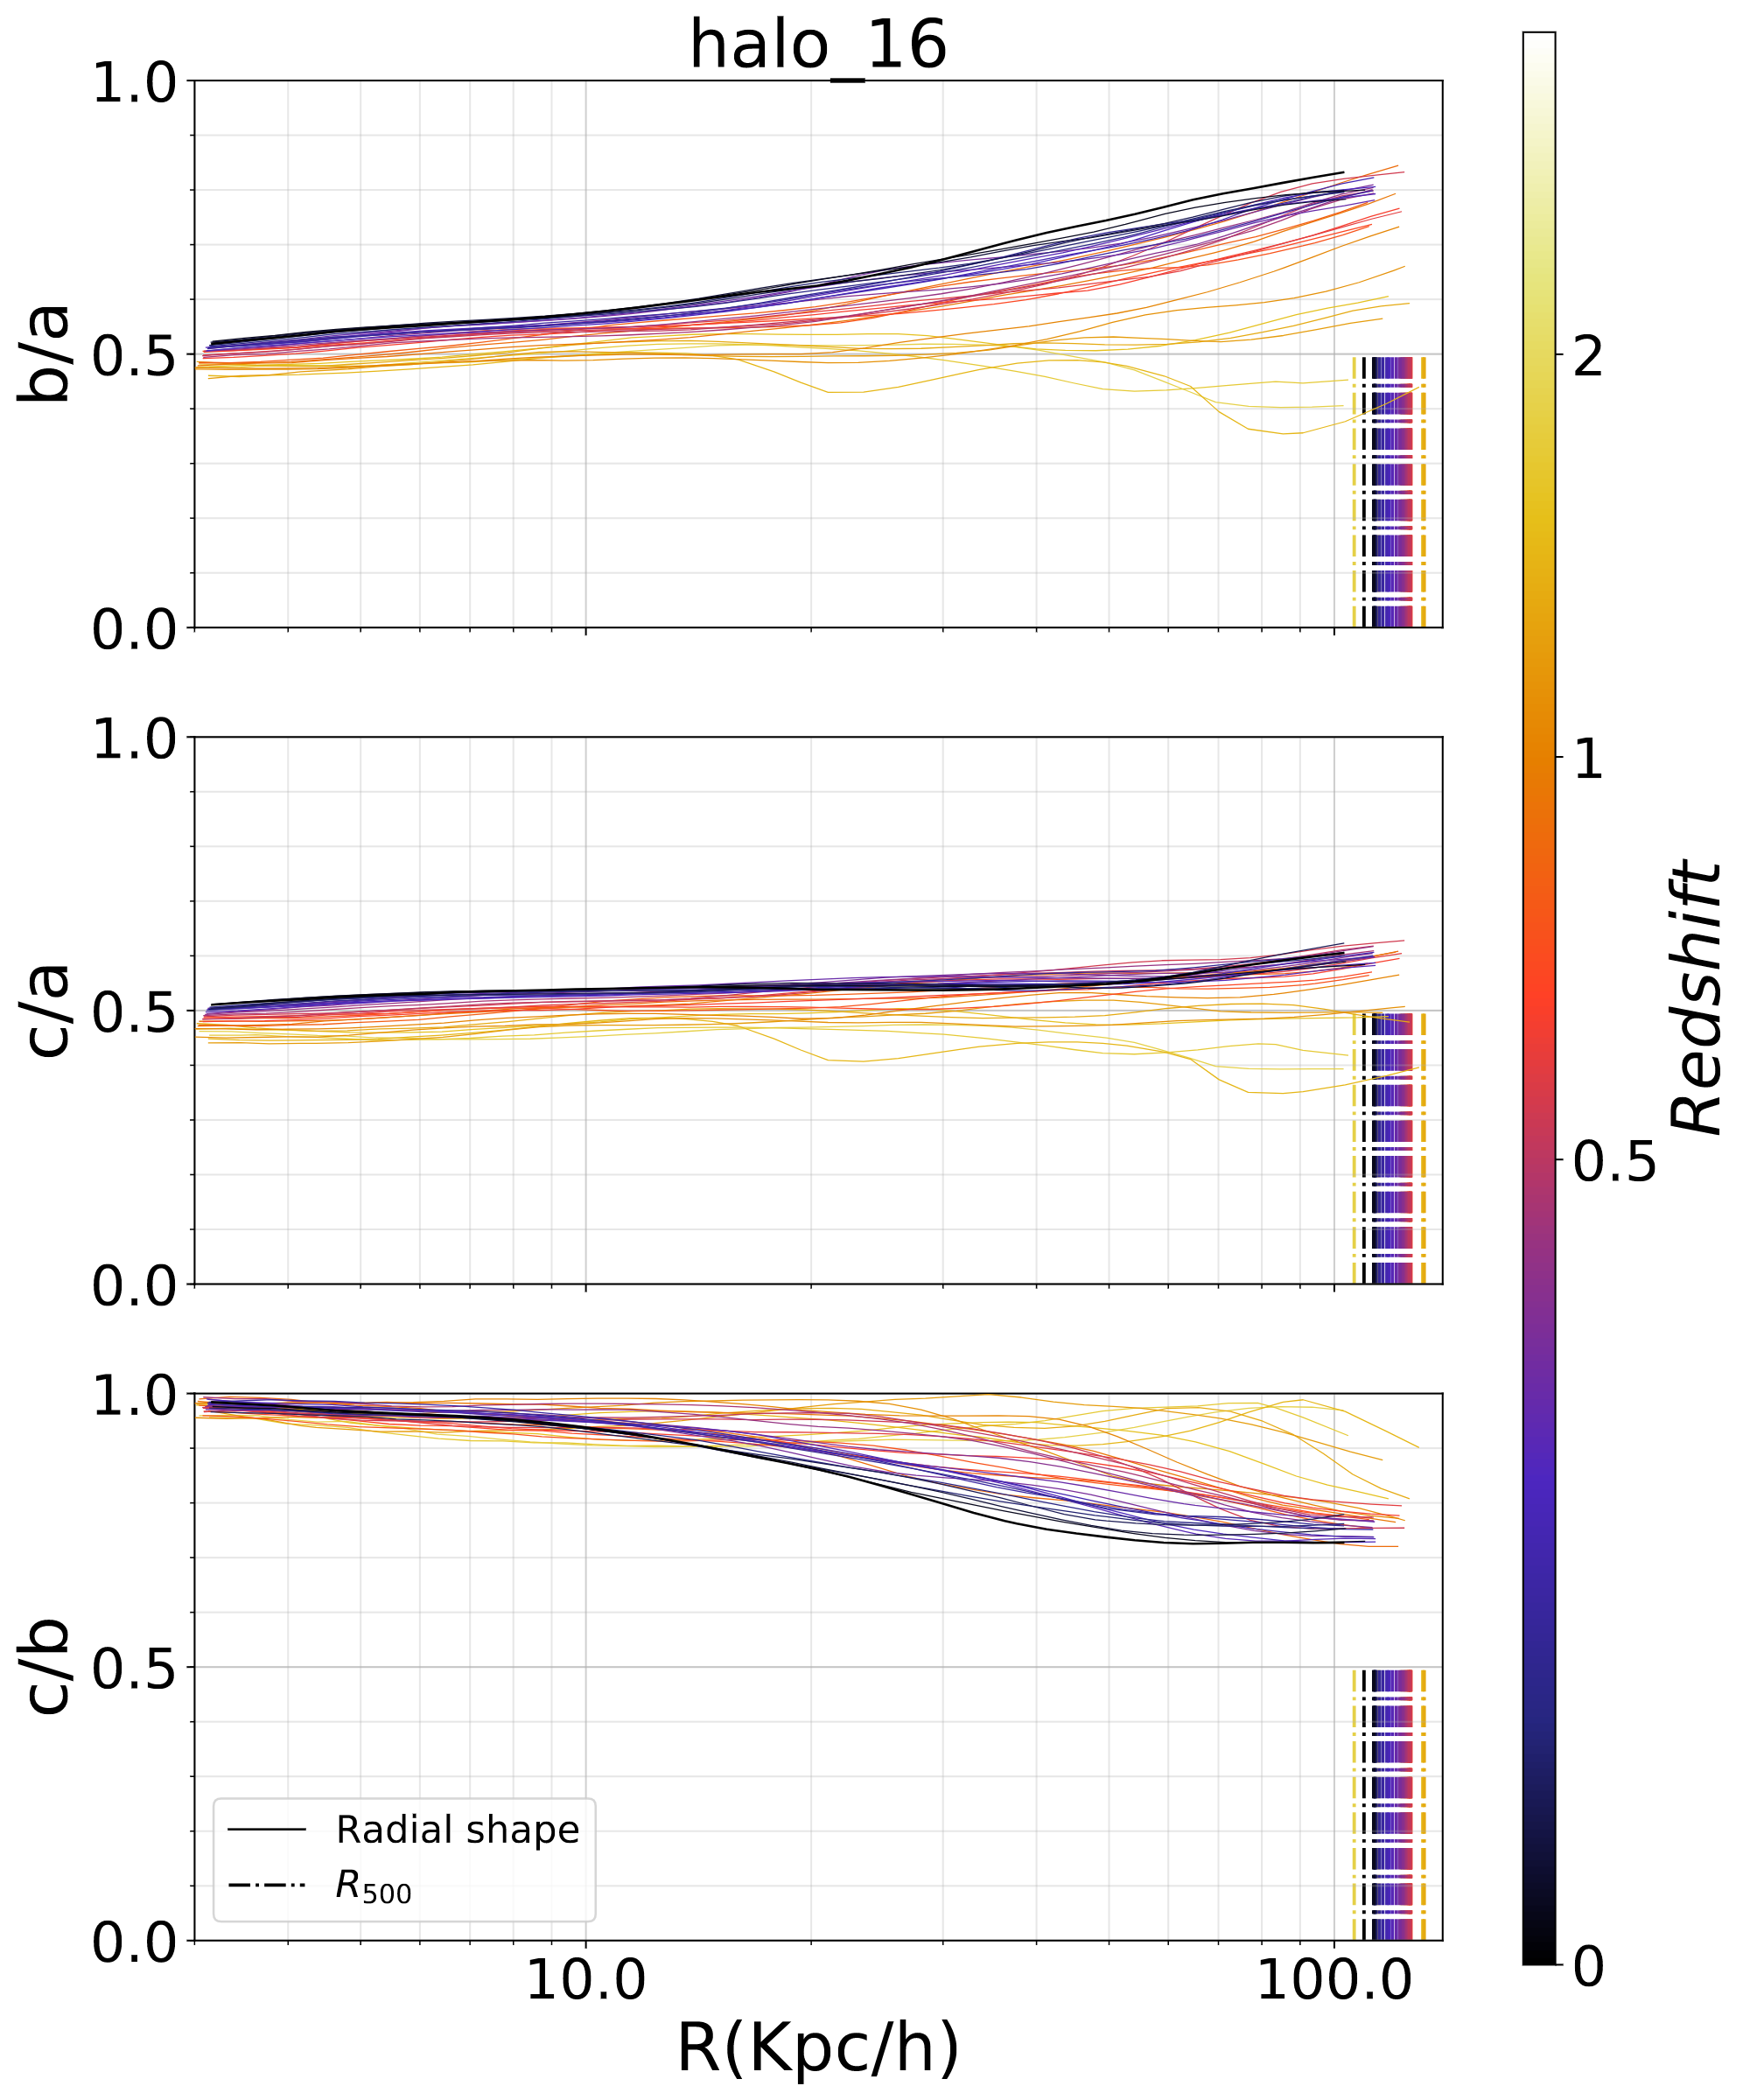
\includegraphics[width=0.5\columnwidth]{./pics/Redshift/halo_16_level3_DM_Z.png}\label{fig:RedshiftDMgood}}
  \hfill
  \subfloat[halo 16 MHD]{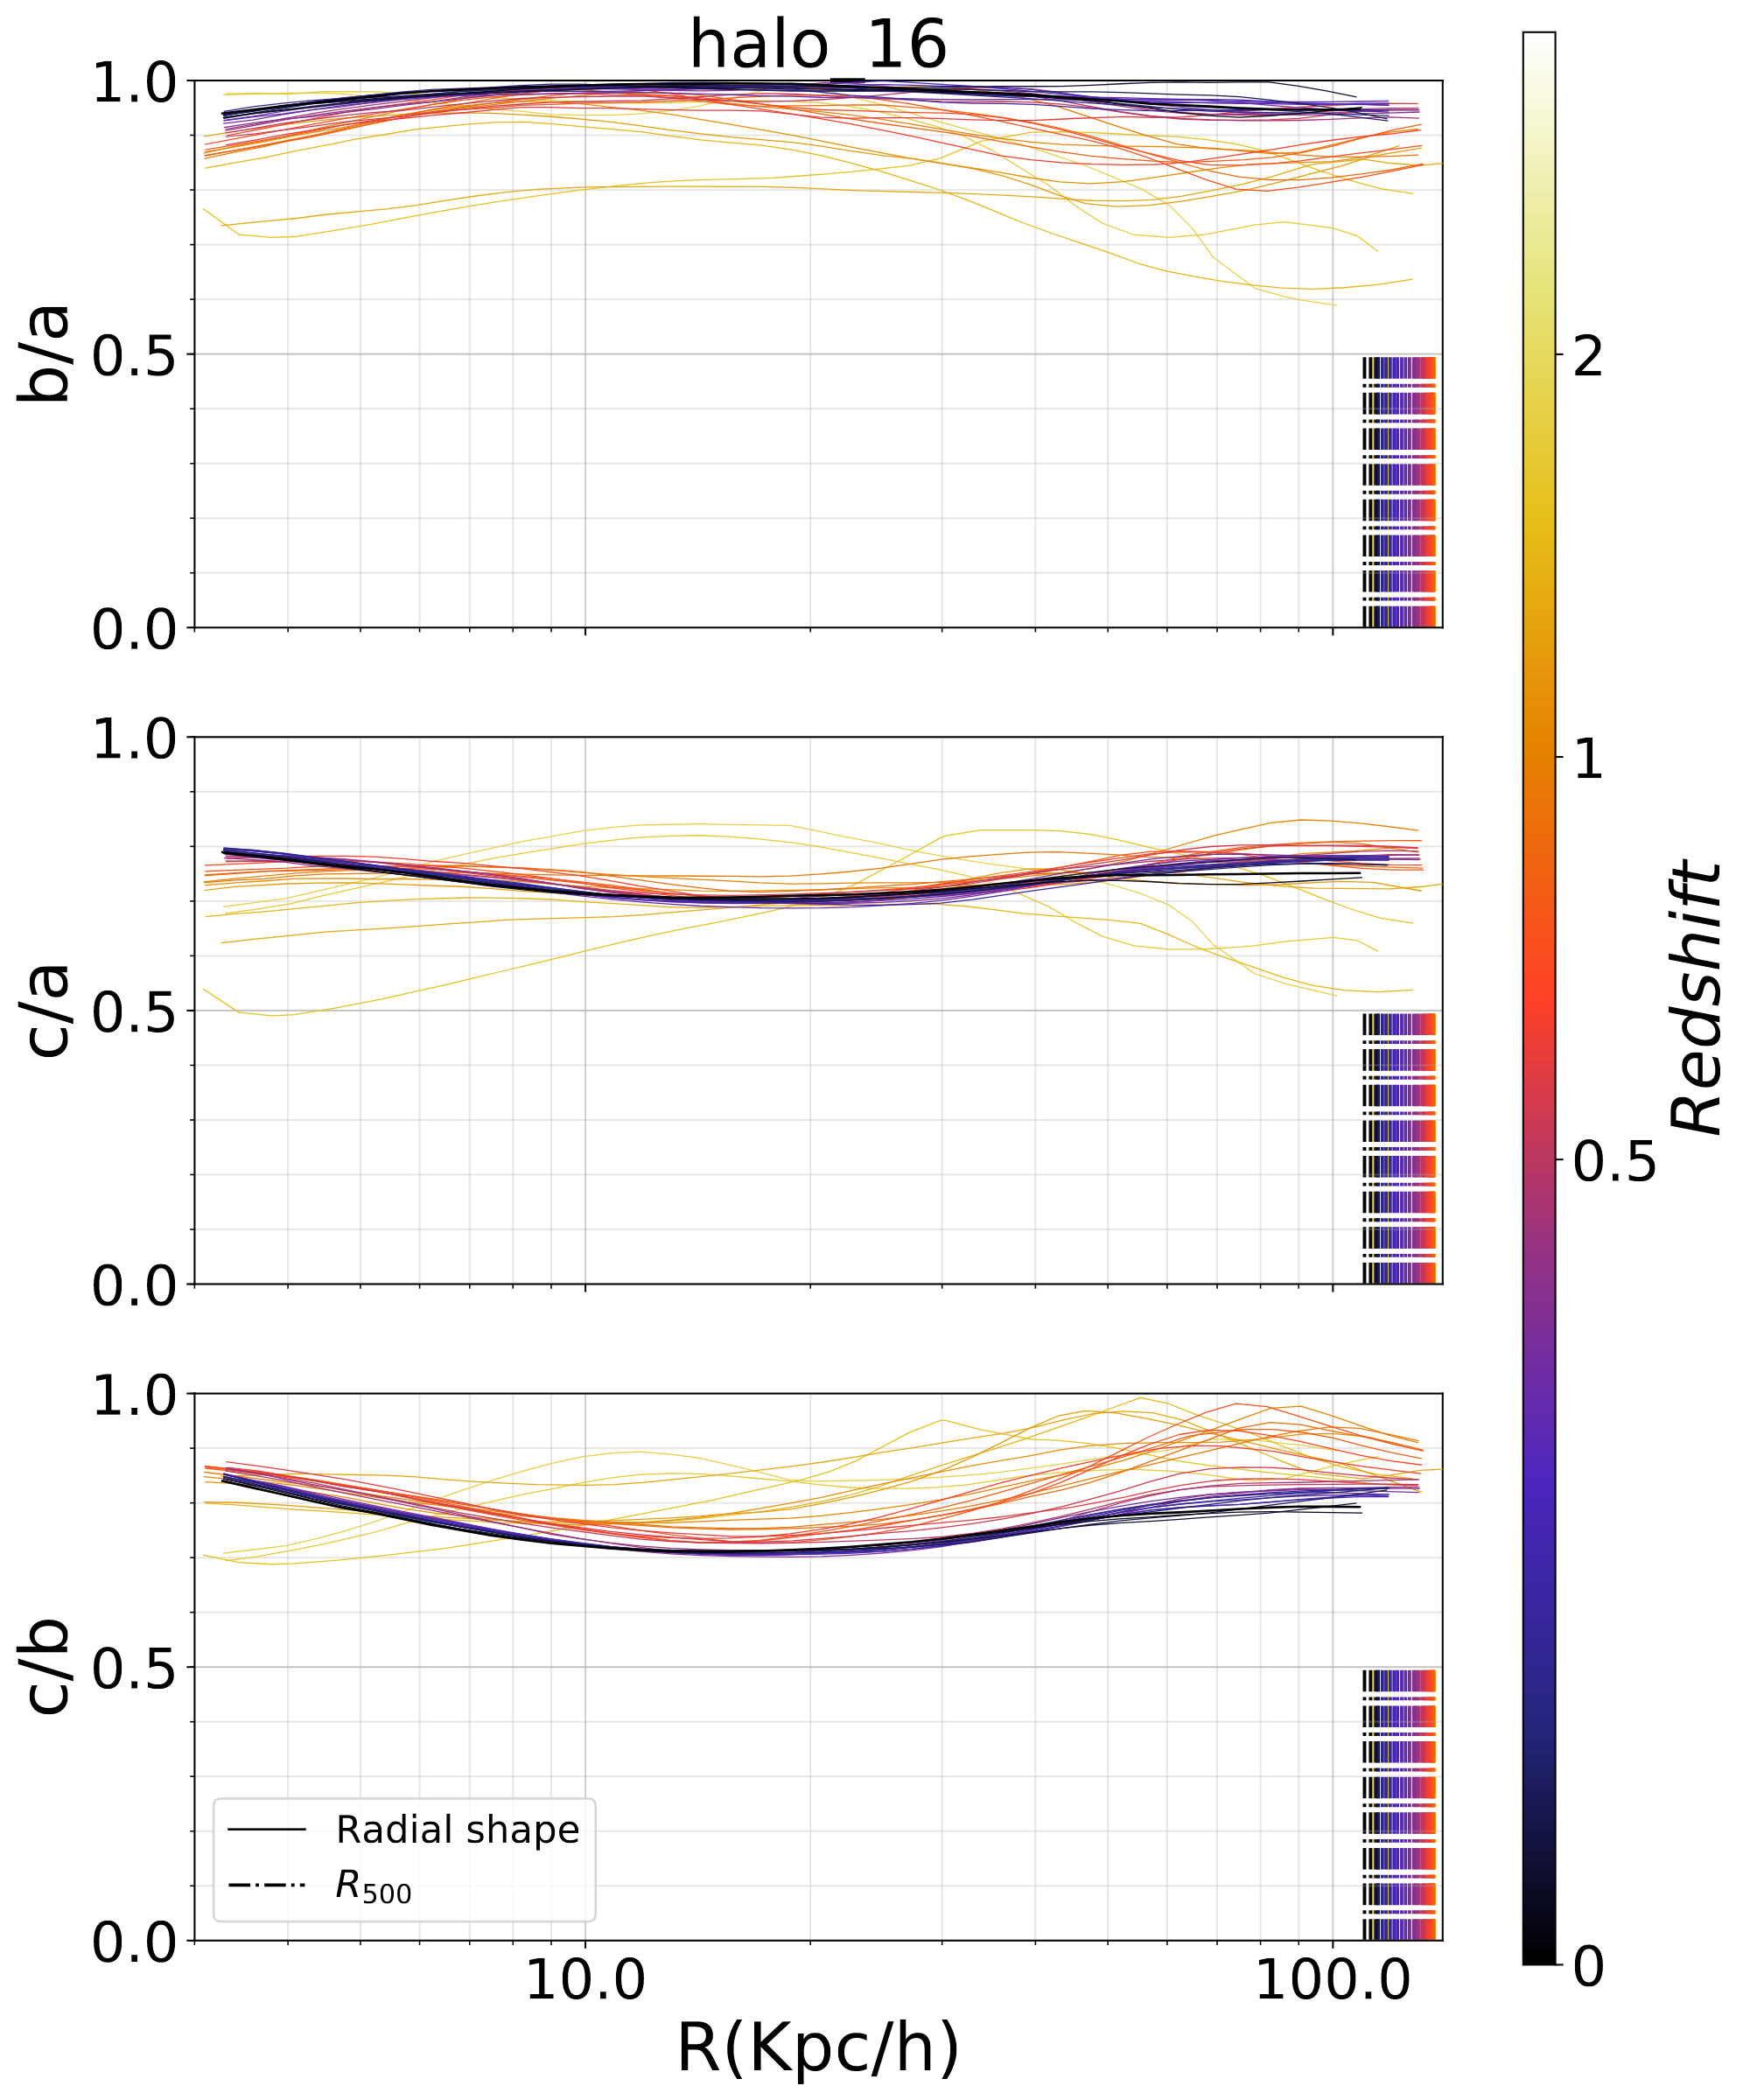
\includegraphics[width=0.5\columnwidth]{./pics/Redshift/halo_16_level3_MHD_Z.png}\label{fig:RedshiftMHDgood}}
  \caption{Example of historic shape conservation in comoving coordinates.\textbf{improve colorbar}}
\end{figure}


\begin{figure}[!ht]
  \centering
  \subfloat[halo 21 DM]{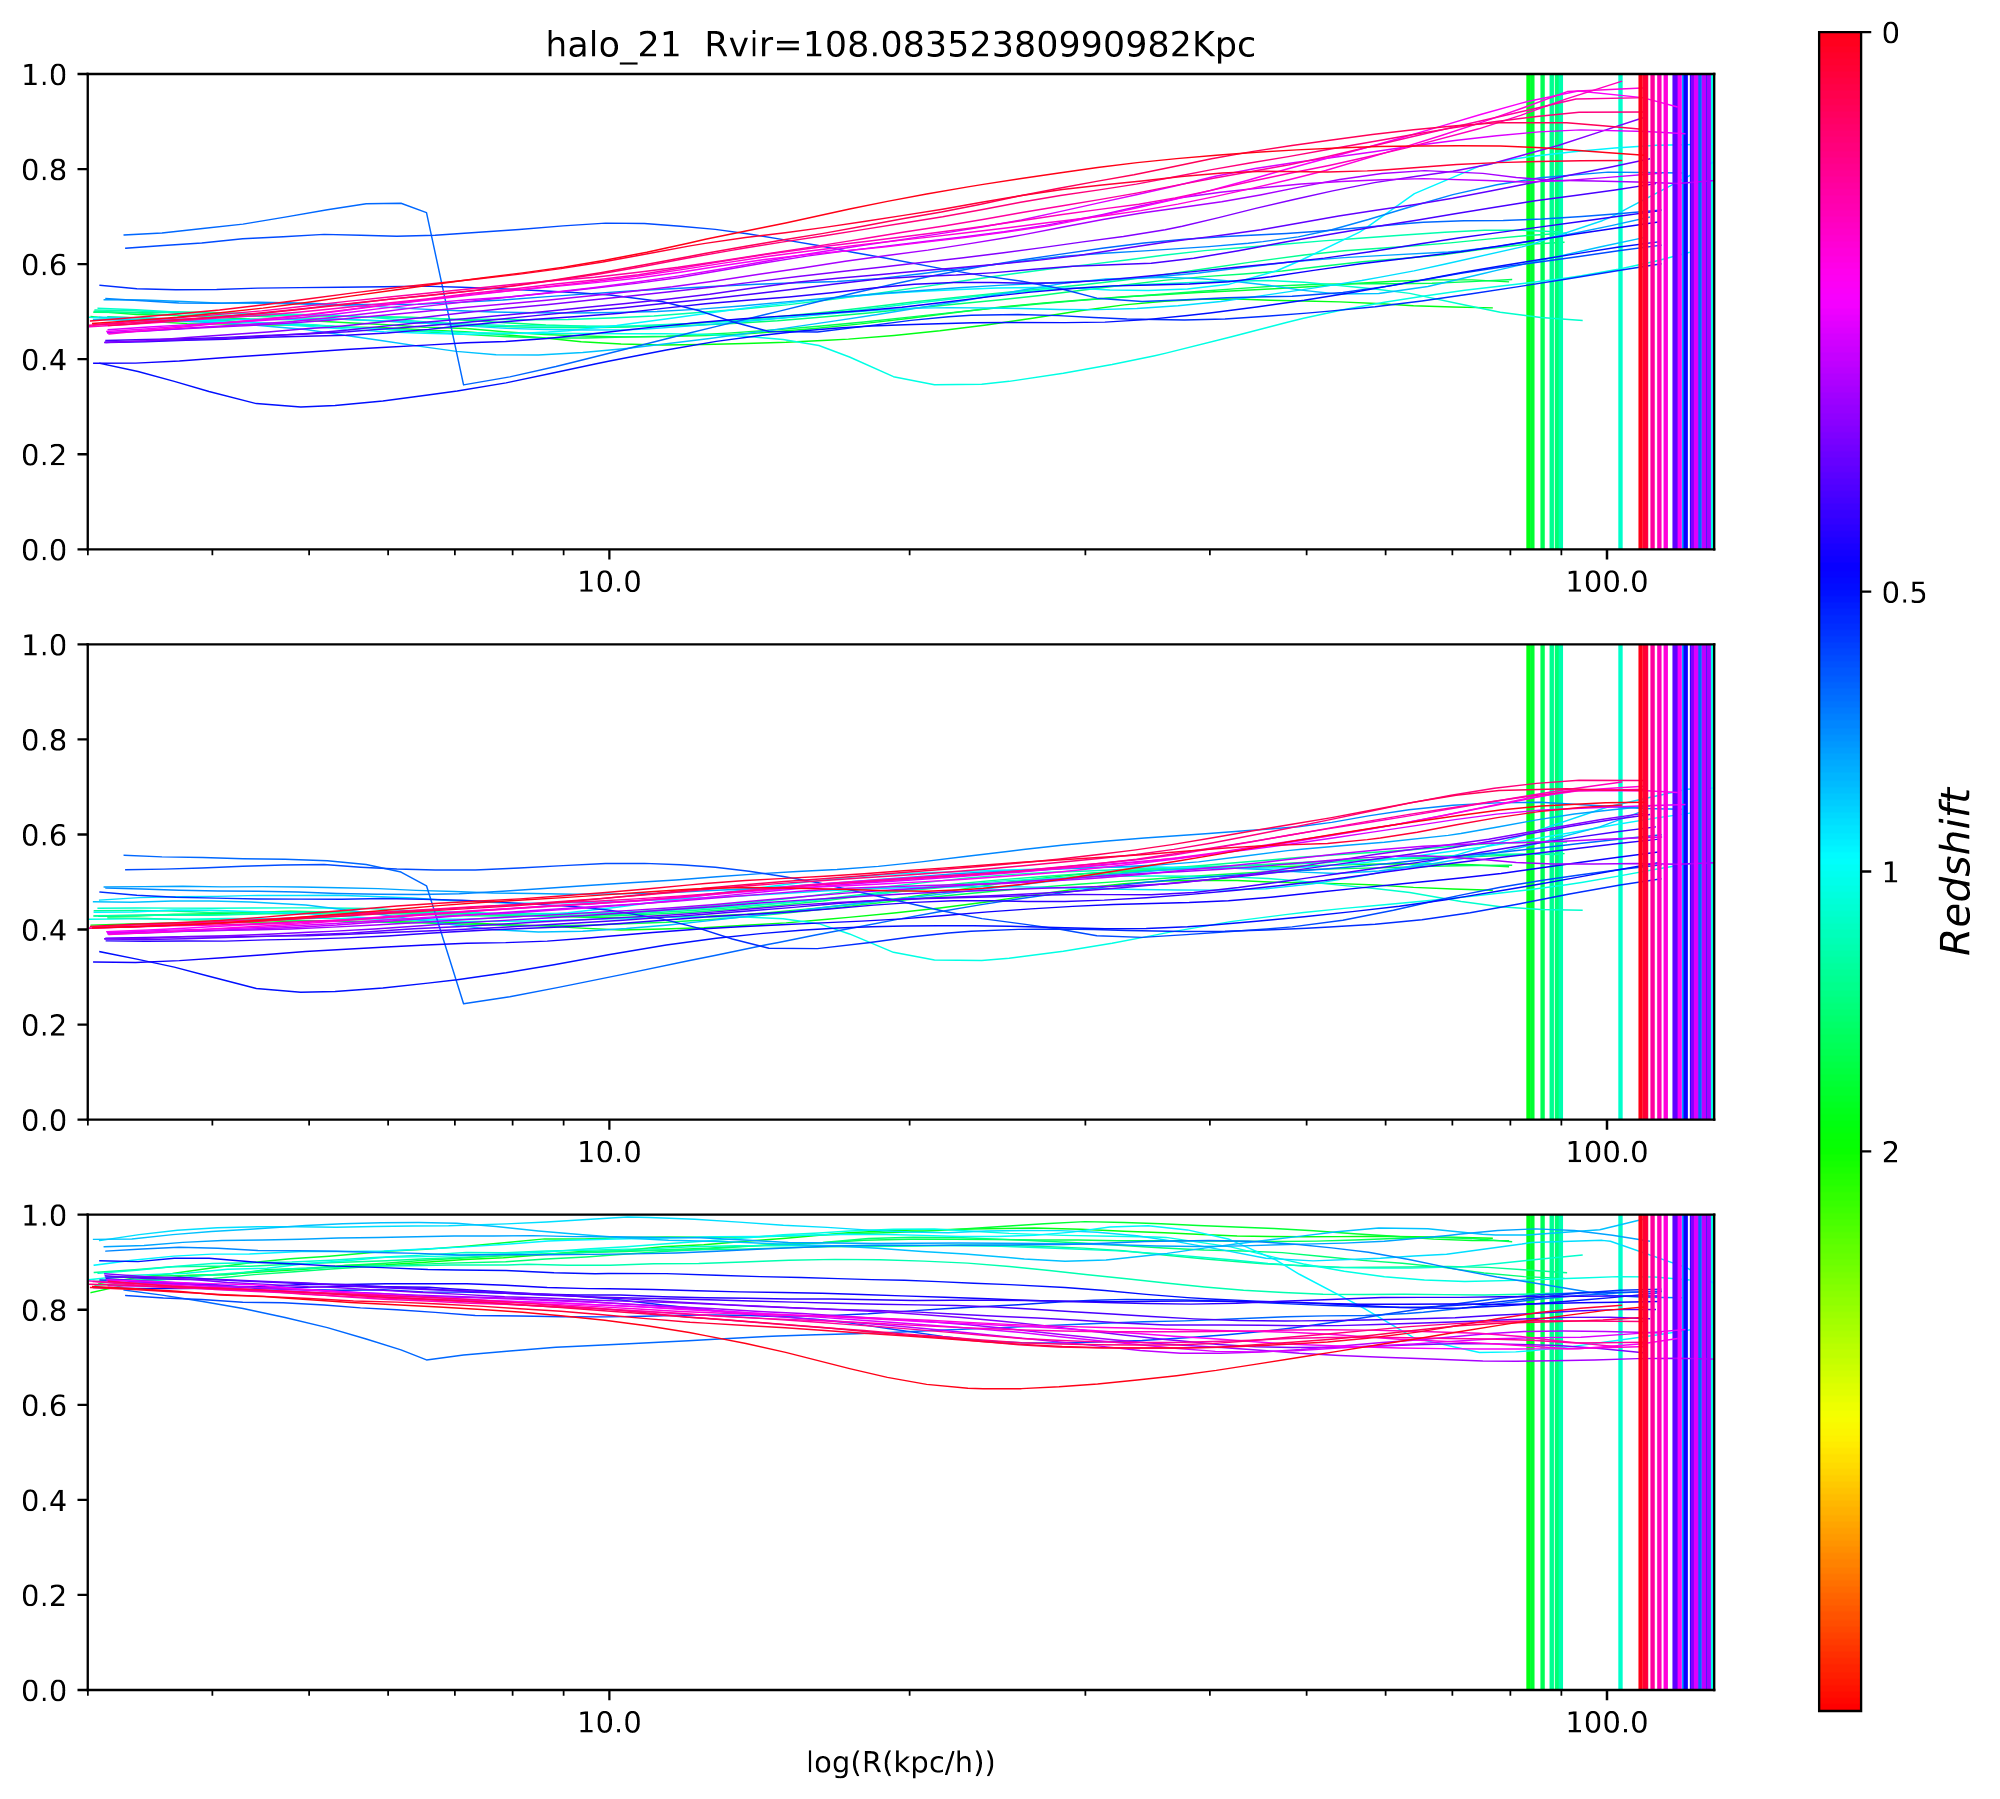
\includegraphics[width=0.5\columnwidth]{./pics/Redshift/halo_21_level3_DM_Z.png}\label{fig:RedshiftDMbad}}
  \hfill
  \subfloat[halo 21 MHD]{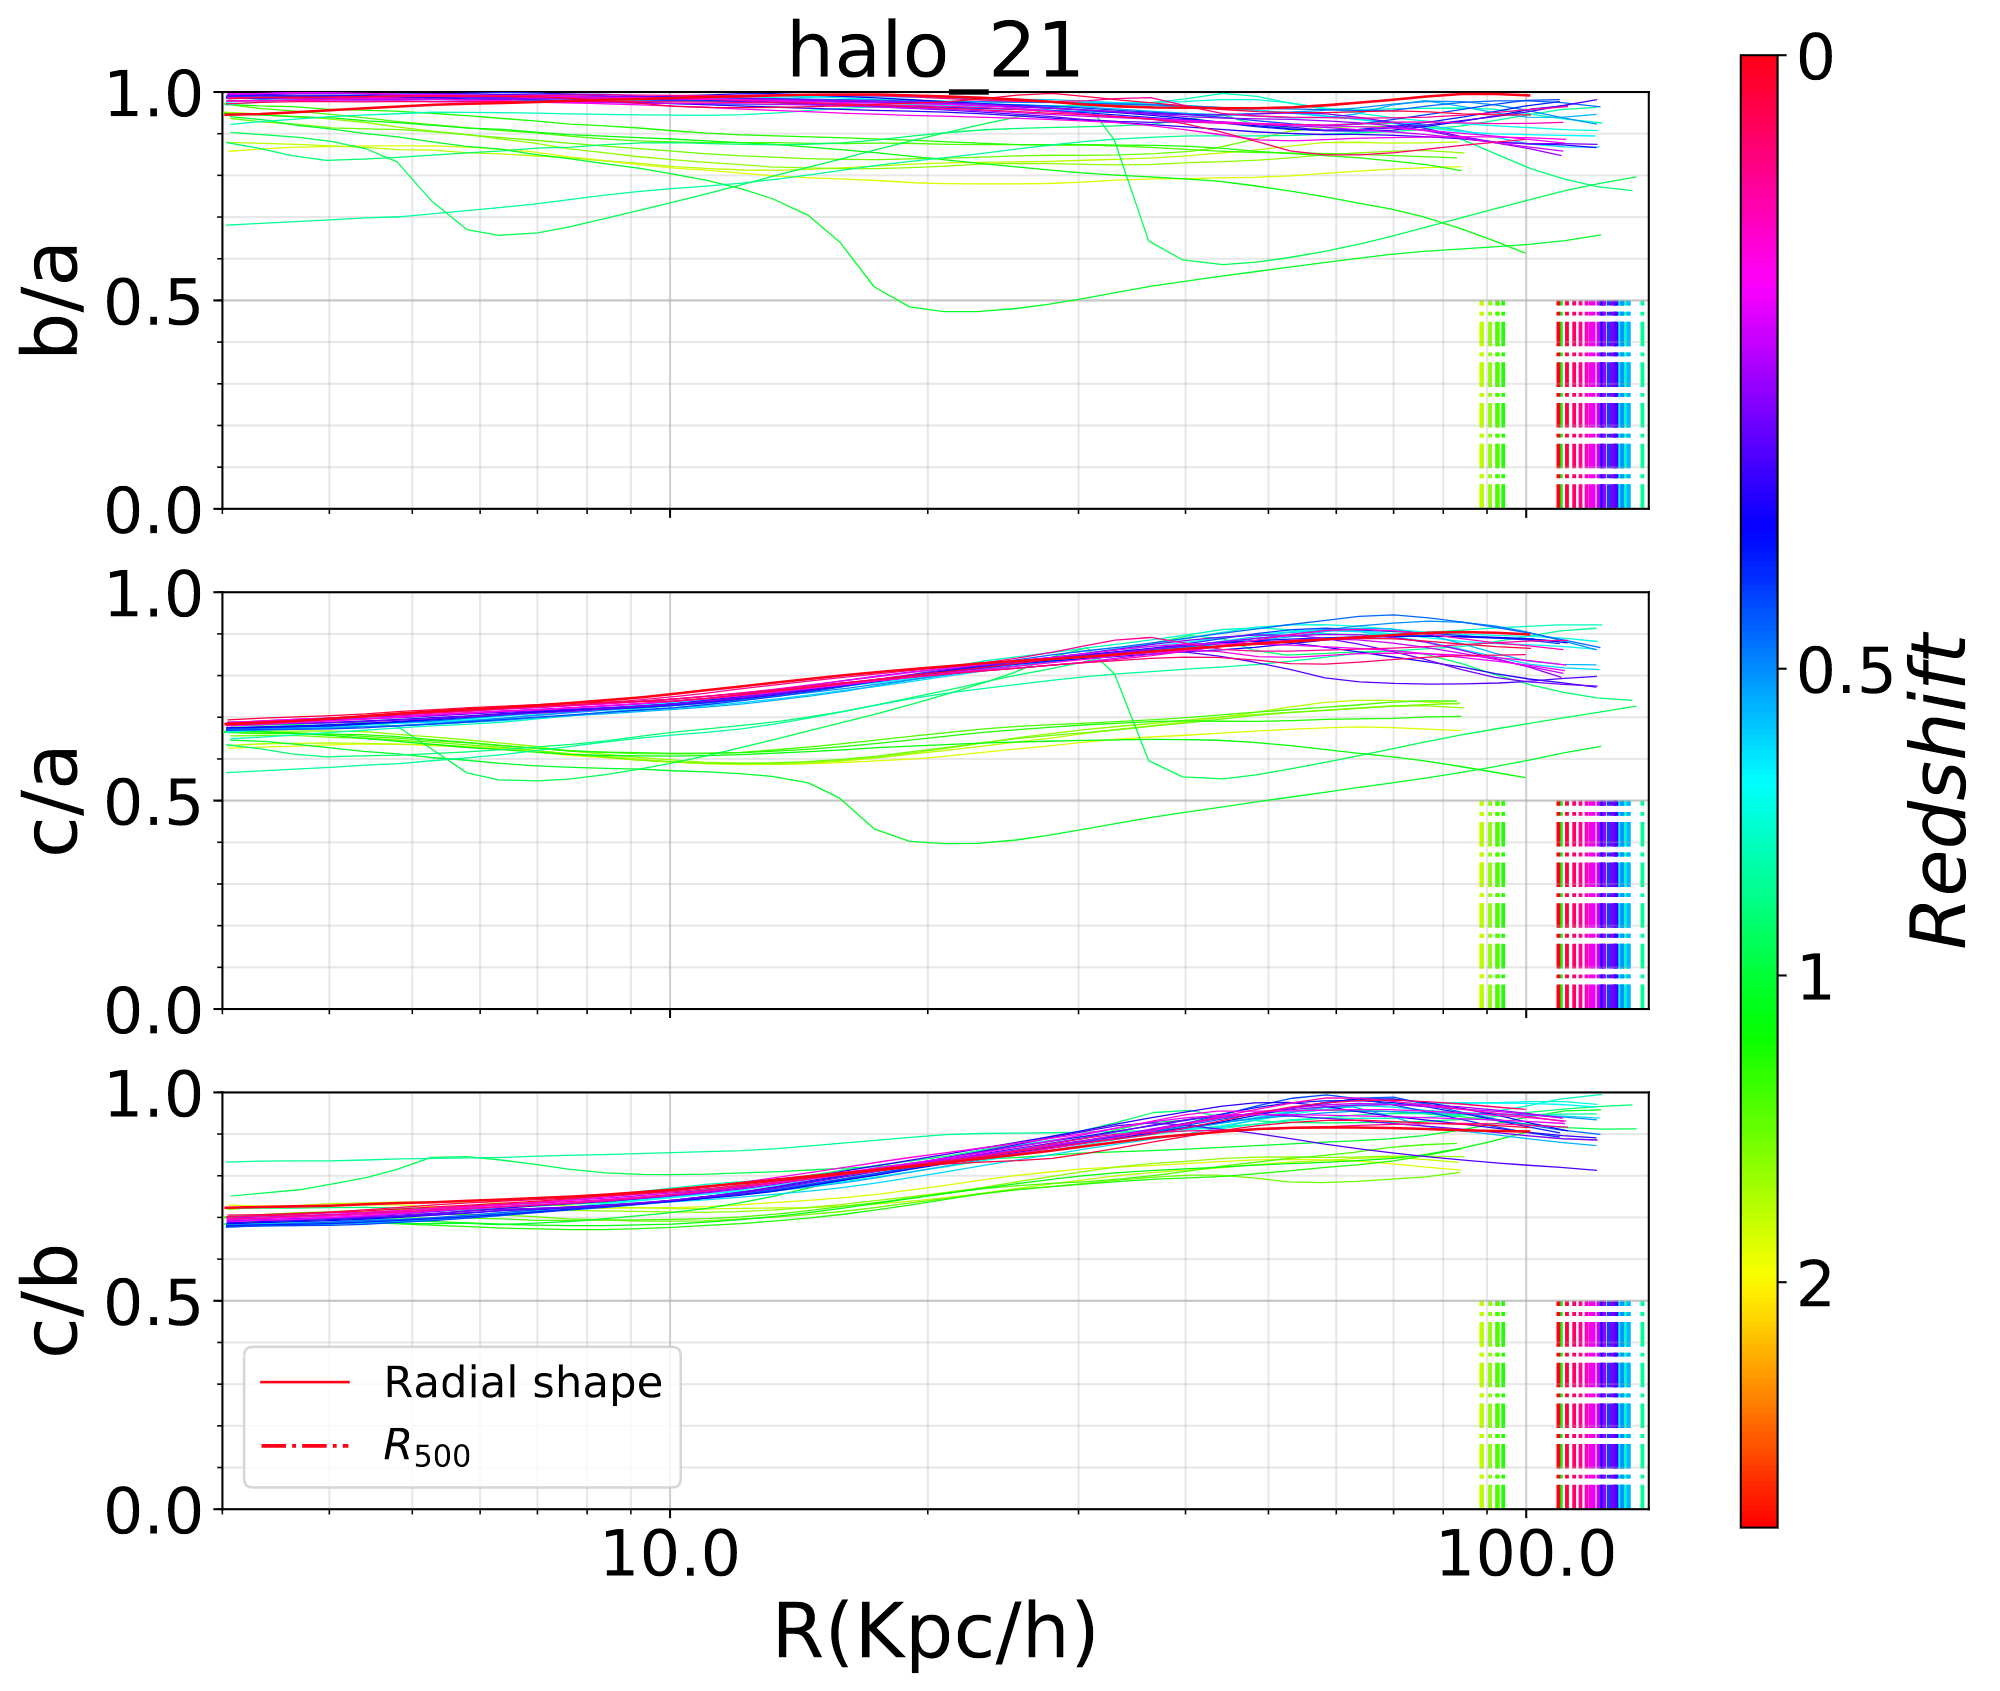
\includegraphics[width=0.5\columnwidth]{./pics/Redshift/halo_21_level3_MHD_Z.png}\label{fig:RedshiftMHDbad}}
  \caption{Example of historic shape disruption in comoving coordinates. The consistency between MHD and DM implies some major-event like a close merger or a collision. The non-continuous red line corresponds to the exact moment of this merging event, which is amplified in MHD.  \textbf{improve colorbar}}
\end{figure}

\begin{figure}[!ht]
  \centering
  \subfloat[halo 16 MHD]{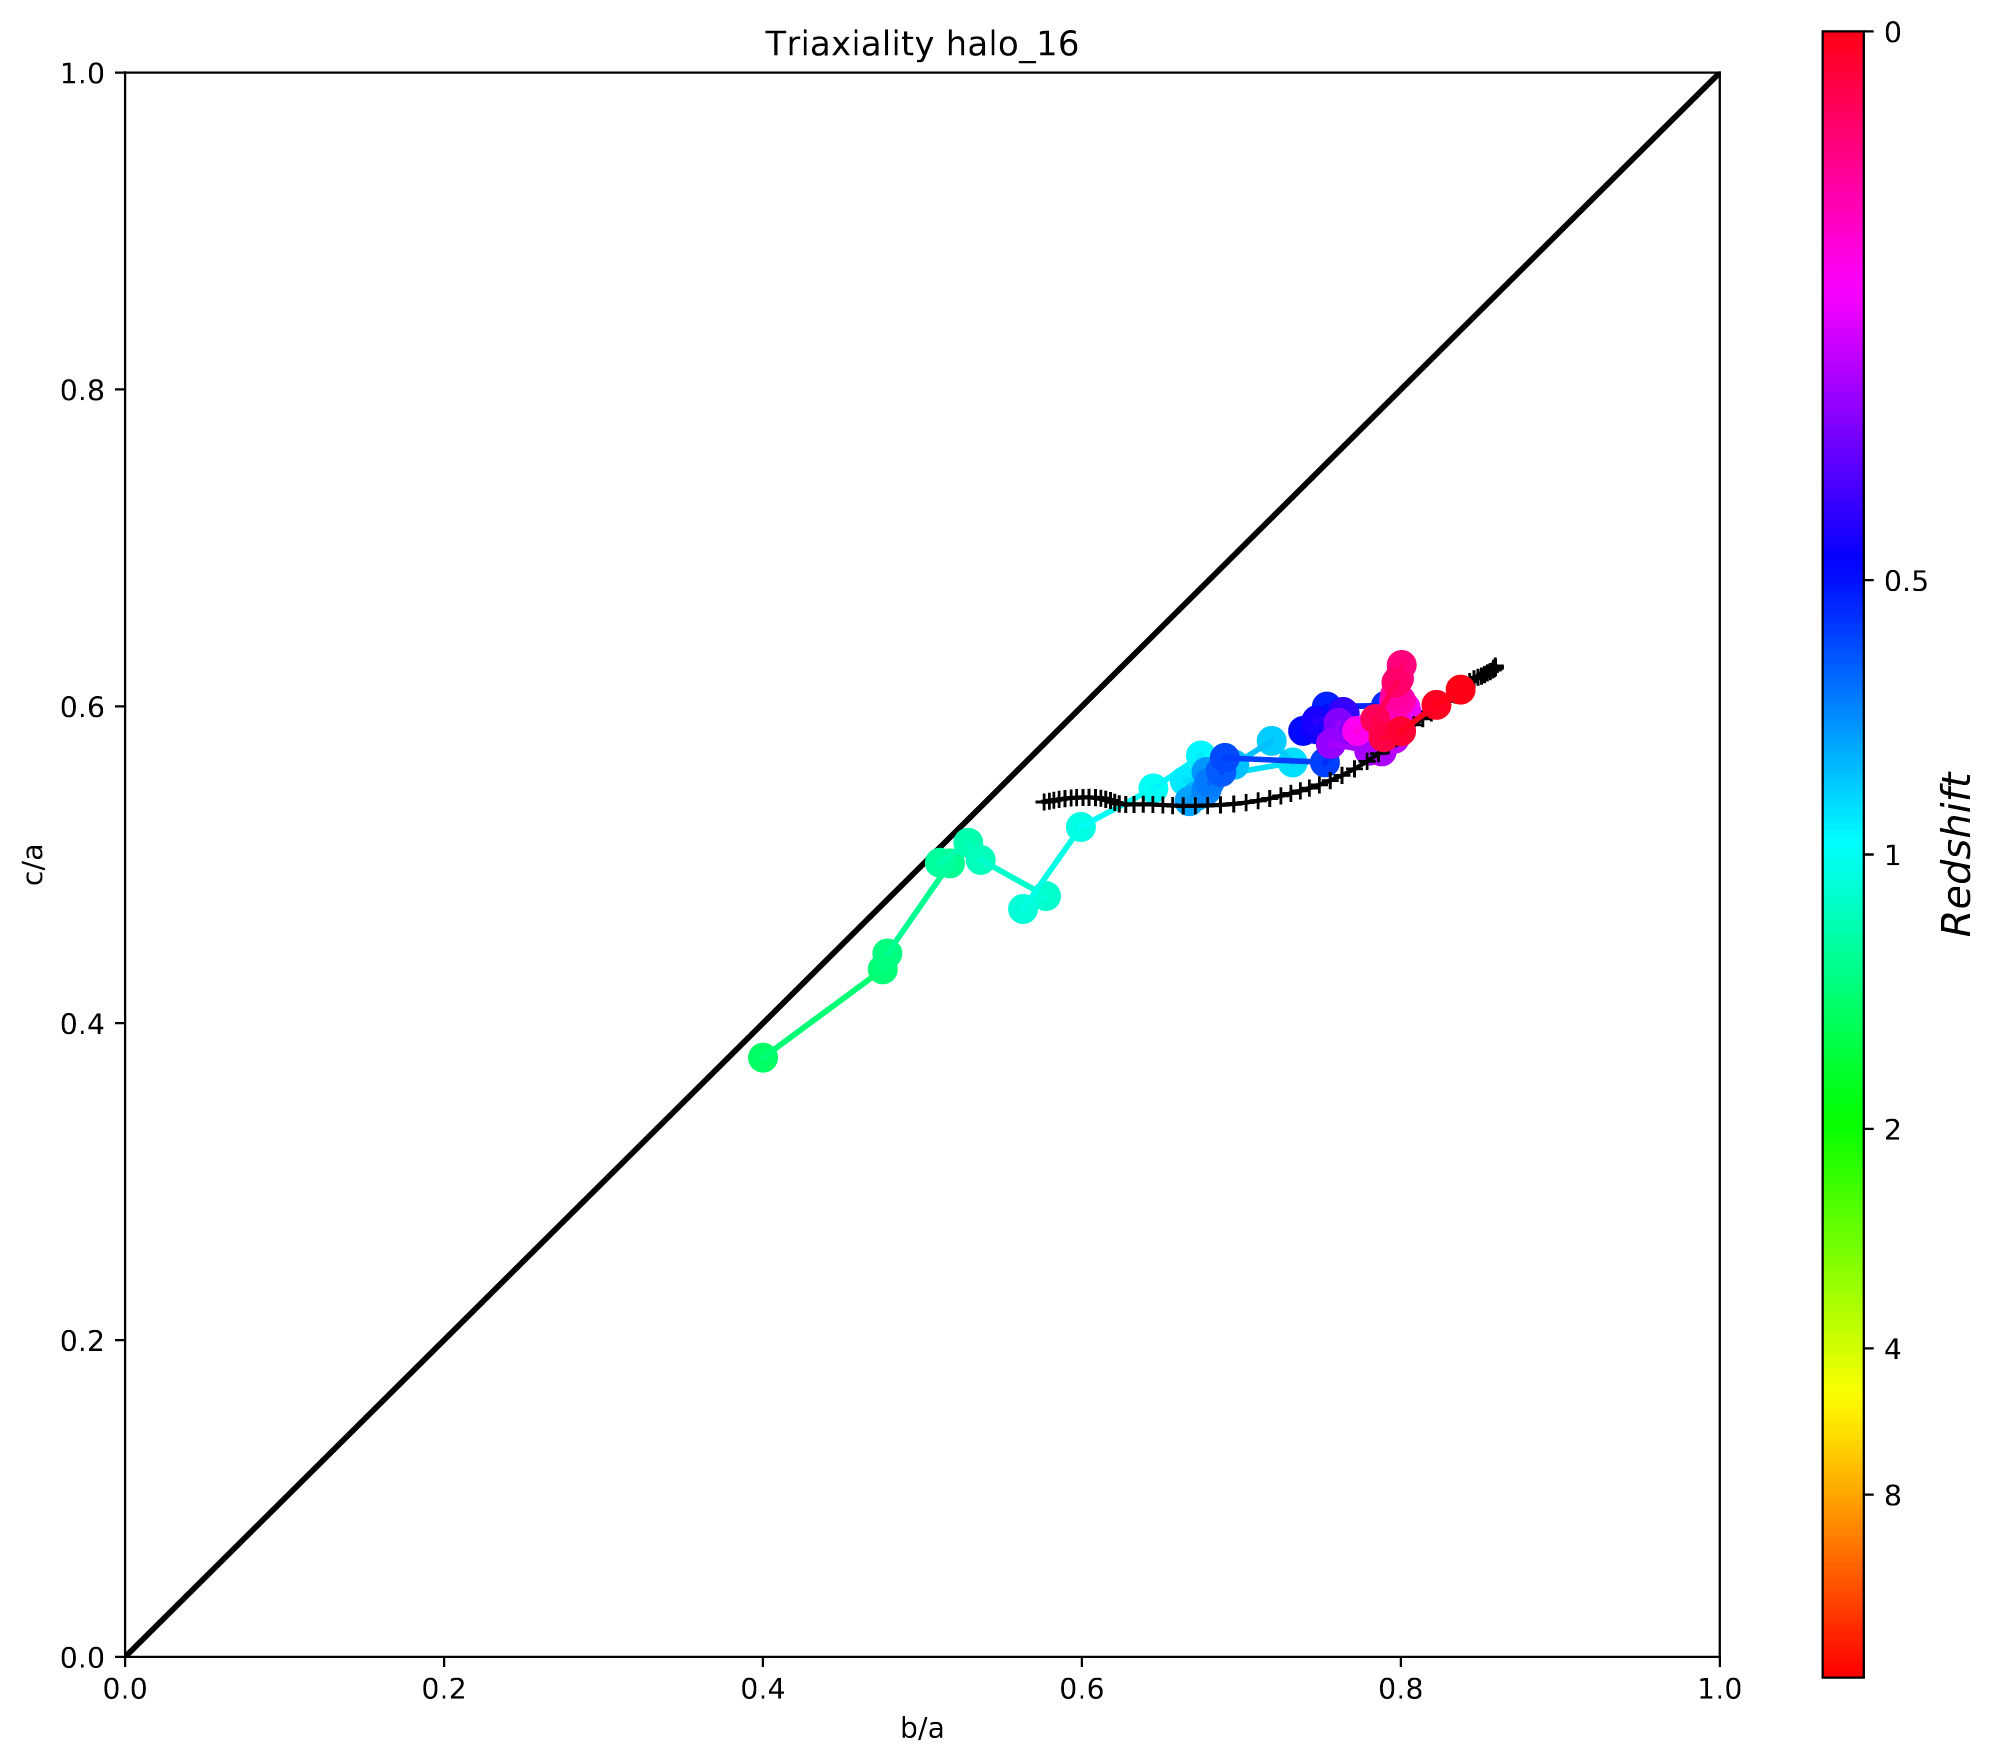
\includegraphics[width=0.5\columnwidth]{./pics/Redshift/halo_16_level3_MHD_Z_Triax.png}\label{fig:RedshiftDMTriax16}}
  \hfill
  \subfloat[halo 21 MHD]{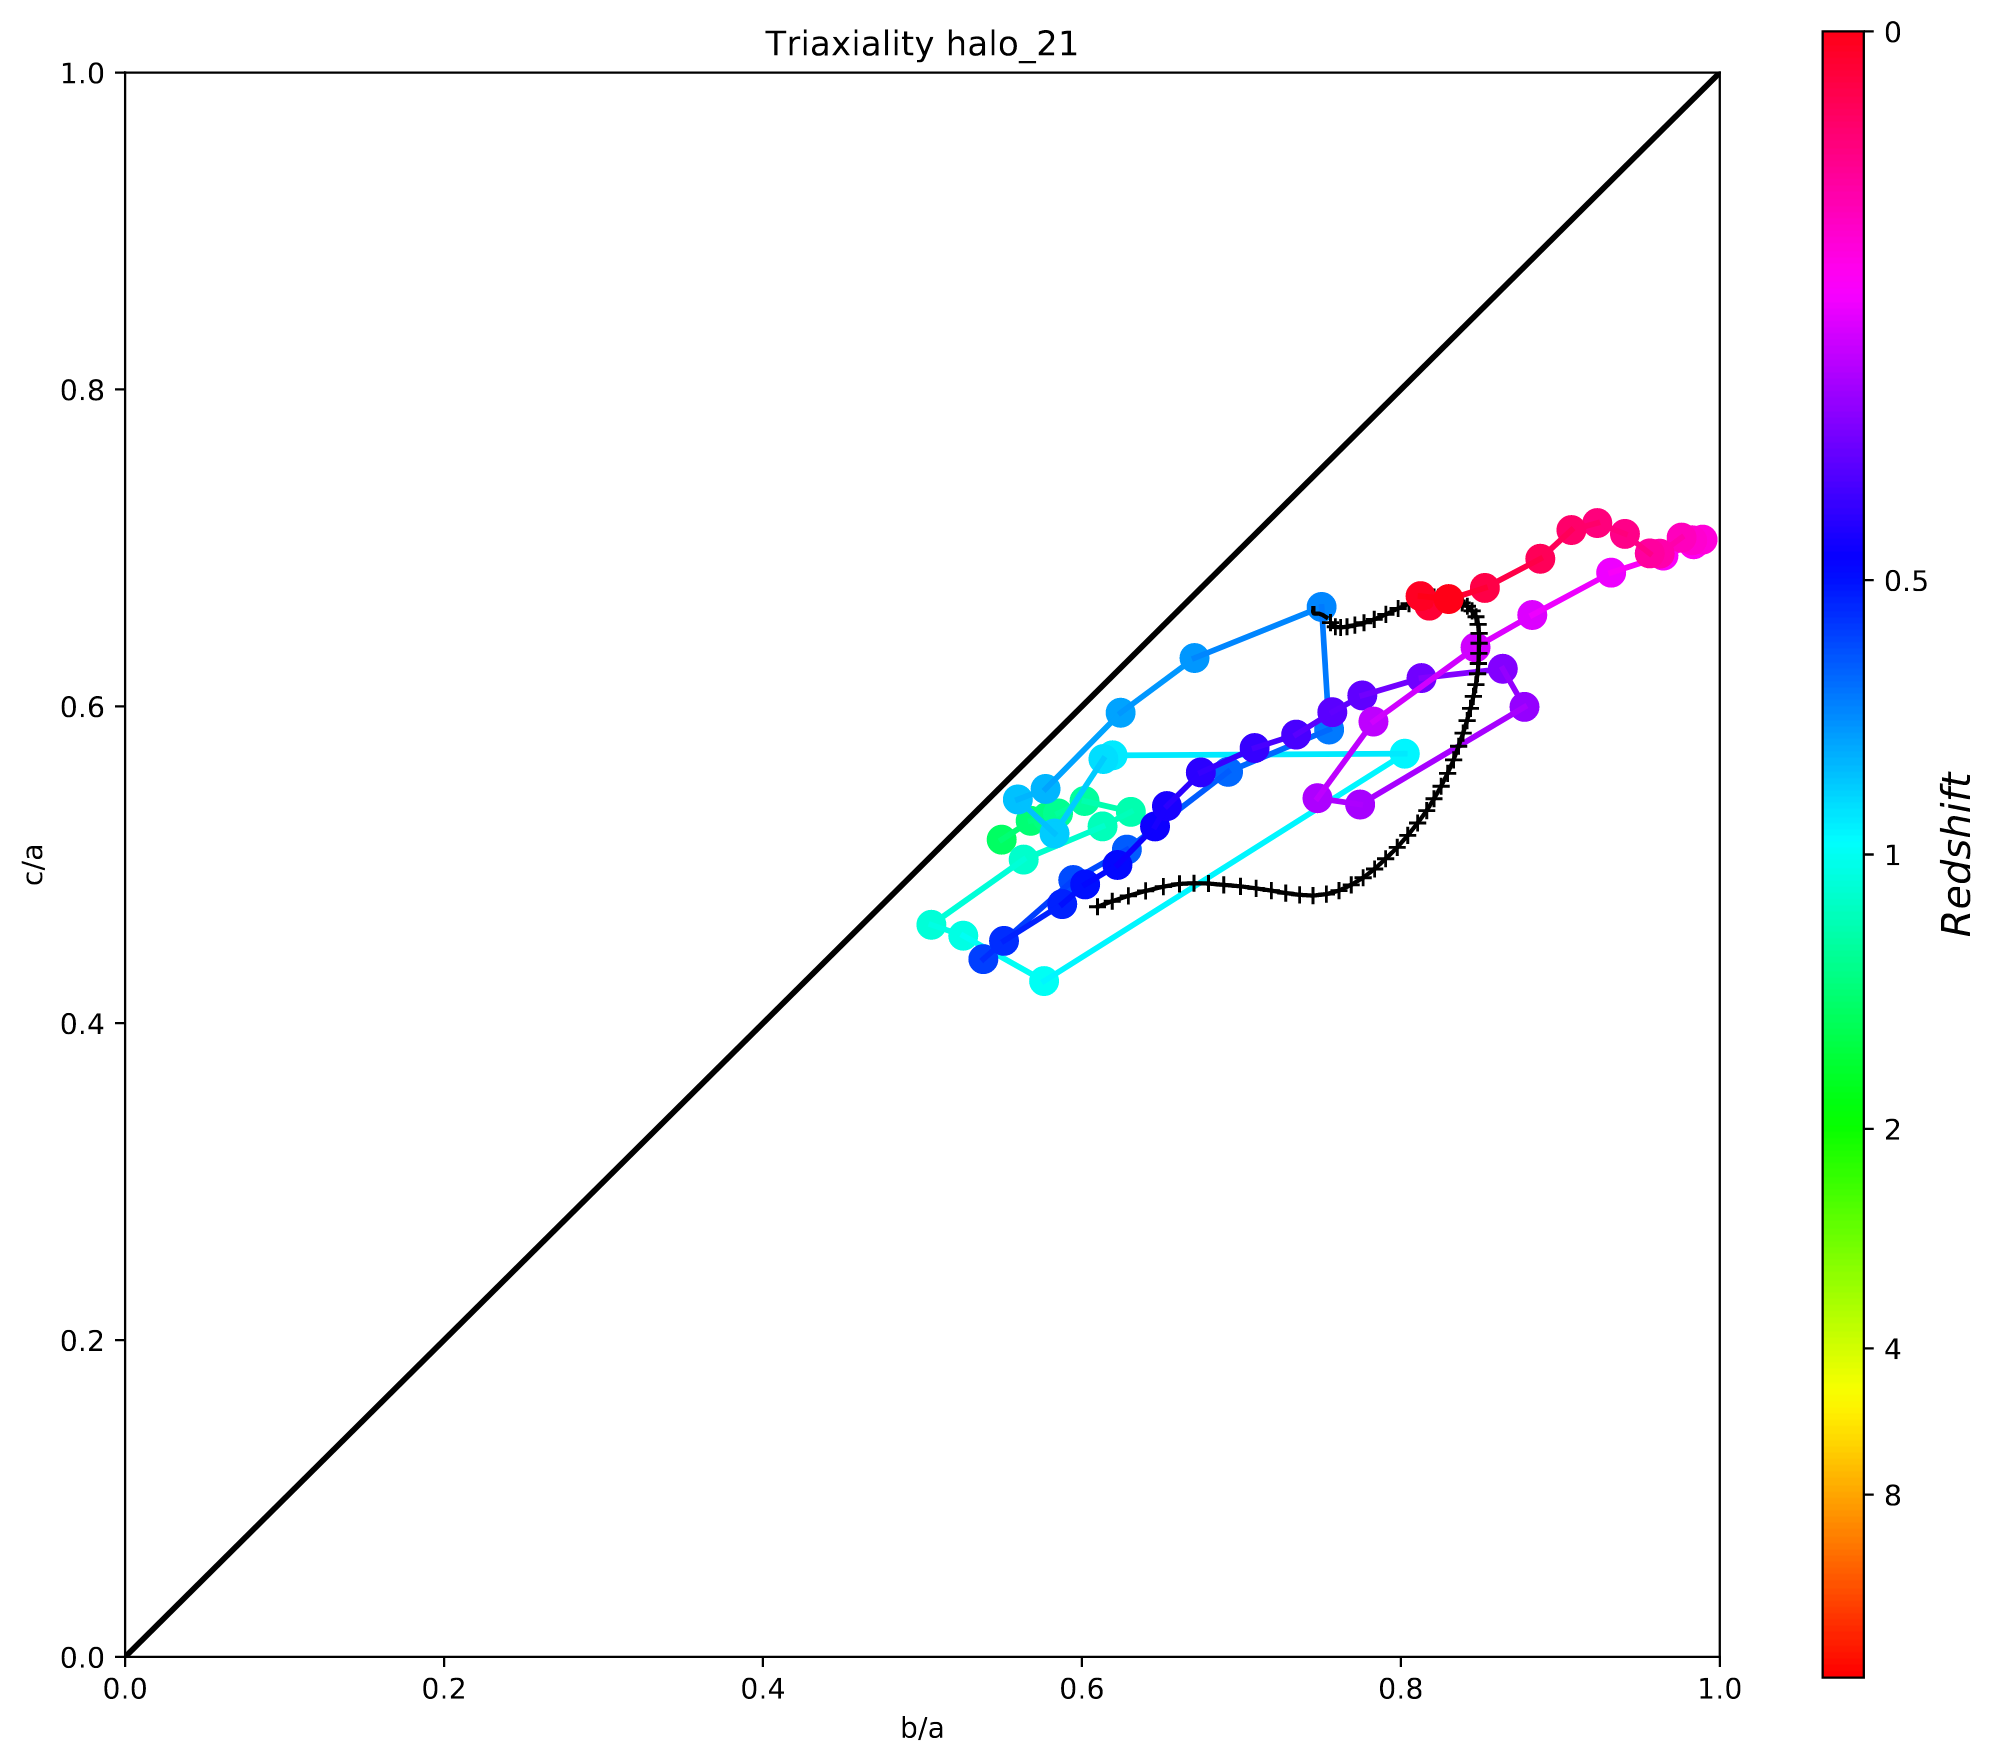
\includegraphics[width=0.5\columnwidth]{./pics/Redshift/halo_21_level3_MHD_Z_Triax.png}\label{fig:RedshiftDMTriax21}}
  \caption{Historic shape Vs radial shape on the Triaxiality plane. The black line represents the radial profile at redshift 0. The colored connected dots represent the shape measured at the virial radius (physical coordinates) at a certain redshift (color)}
\end{figure}




\end{figure}


 
 % Experimental Setup

\chapter{Conclusions}

Our work on the expected shape of DM halos is motivated by various factors. On one hand, obtained insight on the halo shape of full-physics MW-like simulations like Auriga \cite{auriga} may be applied to the improvement of constraints on the DM density field of our MW. This would result in a better comprehension of the behaviour and nature of DM itself. On the other hand, the novelty of gas models in Auriga simulations, which we exploit, makes them unique for the understanding of the effect visible matter on the axial ratios of DM halos. Given the vast work on DM-only simulations, our results could be applied to make more realistic conclusions on these previous studies. Finally, the unique significant sample of 30 high-resolution galaxies from the Auriga project makes our results statistically-supported and may be used to obtain better understanding of random biases that may affect works of this kind.\\  


In this work we use Allgood's method for shape calculation \cite{Allgood_et_al._2006} on the 30-sized set of DM-only and MHD MW-like simulations from the Auriga \cite{auriga} project to verify the results obtained by \cite[Vera-Ciro et al. 2011]{Vera-Ciro_et_al._2011} about the shape of DM halos from Aquarius simulations and obtain more insight about how DM halos behave on MW-like galaxy simulations. Auriga includes consistent models for energetic and accretion feedback from stars and Black Holes and the unique inclusion of magnetic fields. These models worked over a significant set of 30 galaxies evolved with the Arepo code \cite{arepo}, which solves the principal problems of the previous Computational Fluid Dynamics paradigms. All these properties make of Auriga one of the most advanced and precise set of simulations in actuality.\\ 


Taking this into account, we verify that, at $z=0$, DM halos from DM-only and MHD simulations are more oblate/spherical on outer regions and more prolate/triaxial on inner parts. We corroborate this effect in different manners, by obtaining the radial profile of the axial ratios, calculating a triaxiality indicator $T$ and presenting our results on the triaxial plane. Although our results were expected from the work on various cosmological simulations \cite{Frenk_et_al._1988,Dubinski_and_Carlberg_1991,Warren_et_al._1992,Cole_and_Lacey_1996,Hayashi_et_al._2007,Bett_et_al._2007,Vera-Ciro_et_al._2011}, our study is supported with an unprecedented sample of 30 level 4 resolution MW-like simulated galaxies.\\

Taking advantage of the parallel outcome of DM-only and MHD versions of the same galaxies on Auriga, we compare both versions to analyze the effect of the presence of gas on the shape of the DM halos. We find that gas affects the shape at all radii by making the halo more spherical. Furthermore, we demonstrate that this rounding effect is more prominent on the inner regions of the halo. These results are also in agreement with previous studies on this subject \cite{Barnes_and_Hernquist_1996,Springel_et_al._2004,Bryan_et_al._2013}.\\

Vera-Ciro et al. deduced by inspection and showed that there is a correlation between the radial profile of the halo's axial ratios and the historical evolution at a determined radius. We corroborate this fact for DM-only simulations and show the reason for this correlation by calculating the radial shapes at comoving coordinates. We discover that the shape remains more or less unchanged in time once we account for the continuous rounding effect which is shown to be more prominent on the outskirts of the halo, due to the continuous exposure to the inner gravitational potential. This systematic tendency towards sphericity is, together with the pronounced rounding effect at the outskirts of the halo is traduced in a correlation of the historical shape at the virial radius with the radial profile at $z=0$.\\

We conclude our study by stating some interesting questions and proposing further studies on this matter. First, this work may be extended to the analysis of the impact of environmental structures on the shape of the DM halo where it is of special interest the study of the relation of shapes with angular momentum and the orientation of the principal axes of the halo with respect to those determined by cosmic structures. Furthermore, we could make use of the exceptional number of simulated galaxies to address statistical problems such as the verification and improvement of theoretical models that predict the response of DM halos to the presence of matter, like adiabatic contractions \cite{Gnedin_et_al._2004}. \\




 
 
 % Experiment 1

%\input{Chapters/Chapter5} % Experiment 2

%\input{Chapters/Chapter6} % Results and Discussion

%\input{Chapters/Chapter7} % Conclusion

%% ----------------------------------------------------------------
% Now begin the Appendices, including them as separate files

\addtocontents{toc}{\vspace{2em}} % Add a gap in the Contents, for aesthetics

\appendix % Cue to tell LaTeX that the following 'chapters' are Appendices

\chapter{An Appendix}

Lorem ipsum dolor sit amet, consectetur adipiscing elit. Vivamus at pulvinar nisi. Phasellus hendrerit, diam placerat interdum iaculis, mauris justo cursus risus, in viverra purus eros at ligula. Ut metus justo, consequat a tristique posuere, laoreet nec nibh. Etiam et scelerisque mauris. Phasellus vel massa magna. Ut non neque id tortor pharetra bibendum vitae sit amet nisi. Duis nec quam quam, sed euismod justo. Pellentesque eu tellus vitae ante tempus malesuada. Nunc accumsan, quam in congue consequat, lectus lectus dapibus erat, id aliquet urna neque at massa. Nulla facilisi. Morbi ullamcorper eleifend posuere. Donec libero leo, faucibus nec bibendum at, mattis et urna. Proin consectetur, nunc ut imperdiet lobortis, magna neque tincidunt lectus, id iaculis nisi justo id nibh. Pellentesque vel sem in erat vulputate faucibus molestie ut lorem.

Quisque tristique urna in lorem laoreet at laoreet quam congue. Donec dolor turpis, blandit non imperdiet aliquet, blandit et felis. In lorem nisi, pretium sit amet vestibulum sed, tempus et sem. Proin non ante turpis. Nulla imperdiet fringilla convallis. Vivamus vel bibendum nisl. Pellentesque justo lectus, molestie vel luctus sed, lobortis in libero. Nulla facilisi. Aliquam erat volutpat. Suspendisse vitae nunc nunc. Sed aliquet est suscipit sapien rhoncus non adipiscing nibh consequat. Aliquam metus urna, faucibus eu vulputate non, luctus eu justo.

Donec urna leo, vulputate vitae porta eu, vehicula blandit libero. Phasellus eget massa et leo condimentum mollis. Nullam molestie, justo at pellentesque vulputate, sapien velit ornare diam, nec gravida lacus augue non diam. Integer mattis lacus id libero ultrices sit amet mollis neque molestie. Integer ut leo eget mi volutpat congue. Vivamus sodales, turpis id venenatis placerat, tellus purus adipiscing magna, eu aliquam nibh dolor id nibh. Pellentesque habitant morbi tristique senectus et netus et malesuada fames ac turpis egestas. Sed cursus convallis quam nec vehicula. Sed vulputate neque eget odio fringilla ac sodales urna feugiat.

Phasellus nisi quam, volutpat non ullamcorper eget, congue fringilla leo. Cras et erat et nibh placerat commodo id ornare est. Nulla facilisi. Aenean pulvinar scelerisque eros eget interdum. Nunc pulvinar magna ut felis varius in hendrerit dolor accumsan. Nunc pellentesque magna quis magna bibendum non laoreet erat tincidunt. Nulla facilisi.

Duis eget massa sem, gravida interdum ipsum. Nulla nunc nisl, hendrerit sit amet commodo vel, varius id tellus. Lorem ipsum dolor sit amet, consectetur adipiscing elit. Nunc ac dolor est. Suspendisse ultrices tincidunt metus eget accumsan. Nullam facilisis, justo vitae convallis sollicitudin, eros augue malesuada metus, nec sagittis diam nibh ut sapien. Duis blandit lectus vitae lorem aliquam nec euismod nisi volutpat. Vestibulum ornare dictum tortor, at faucibus justo tempor non. Nulla facilisi. Cras non massa nunc, eget euismod purus. Nunc metus ipsum, euismod a consectetur vel, hendrerit nec nunc.	% Appendix Title

%\input{Appendices/AppendixB} % Appendix Title

%\input{Appendices/AppendixC} % Appendix Title

\addtocontents{toc}{\vspace{2em}}  % Add a gap in the Contents, for aesthetics
\backmatter

%% ----------------------------------------------------------------
\label{Bibliography}
\lhead{\emph{Bibliography}}  % Change the left side page header to "Bibliography"
\bibliographystyle{unsrtnat}  % Use the "unsrtnat" BibTeX style for formatting the Bibliography
\bibliography{Bibliography}  % The references (bibliography) information are stored in the file named "Bibliography.bib"

\end{document}  % The End
%% ----------------------------------------------------------------
